%%%%%%% Document class and page layout %%%%%%%
\documentclass[a4paper,12pt]{book}
\raggedbottom

%%%%%%% Importing packages %%%%%%%
\usepackage{layout}
\usepackage{calc}
\usepackage{setspace}
\usepackage{graphicx}
\usepackage{amsmath}
\usepackage{float}
\usepackage{caption}
\usepackage{subcaption}
\usepackage{tikz}
\usepackage{subcaption}
\usepackage{natbib}
% \setlength{\parindent}{0cm}
\graphicspath{{images/}{../images/}}


%%%%%%% Clickable links %%%%%%%
\usepackage{hyperref}
\hypersetup{
	colorlinks,
	citecolor=blue,
	filecolor=blue,
	linkcolor=blue,
	urlcolor=blue
}

%%%%%% Tables %%%%%%%%
\usepackage{booktabs}
\usepackage{multirow}
\usepackage[normalem]{ulem}
\useunder{\uline}{\ul}{}
\usepackage{float}

%%%%%%% Word Counting %%%%%%%
\newcommand{\detailtexcount}[1]{%
  \immediate\write18{texcount -merge -sum -q #1.tex output.bbl > #1.wcdetail }%
  \verbatiminput{#1.wcdetail}%
}
\newcommand{\quickwordcount}[1]{%
  \immediate\write18{texcount -1 -sum -merge -q #1.tex output.bbl > #1-words.sum }%
  \input{#1-words.sum} words%
}
\newcommand{\quickcharcount}[1]{%
  \immediate\write18{texcount -1 -sum -merge -char -q #1.tex output.bbl > #1-chars.sum }%
  \input{#1-chars.sum} characters (not including spaces)%
}


%%%%%%% Page styles %%%%%%%
\setlength{\hoffset}{-1in} \setlength{\oddsidemargin}{40mm} \setlength{\evensidemargin}{30mm}
\setlength{\textwidth}{\paperwidth-\oddsidemargin-\evensidemargin} \onehalfspacing
% \setlength{\parskip}{1cm plus 4mm minus 3mm}


%%%%%%% For the multiple files %%%%%%%
\usepackage{subfiles} % Best loaded last in the preamble

%%%%%%% Document starts here
\begin{document}

%%%%%%% Title Page %%%%%%%
\frontmatter
\begin{titlepage} \vspace{20mm} \centering
{\Huge\textbf{Quantifying the Impact of Atmospheric and Oceanic Processes on the behaviour of Sea Ice in Antarctica}\par}  \vspace{20mm} {\Large Hamish Jelleyman} \\ \vspace{20mm} 
\includegraphics{Images/UoA_Crest.eps} \\ \vspace{20mm} A thesis submitted in fulfilment of the requirements \\ for the degree of Master of Science in Physics \\ \vspace{20mm} The University of Auckland \\ 2020
\end{titlepage}

\chapter*{Abstract}
\chapter*{Acknowledgements}

\tableofcontents
\listoffigures
\listoftables

%%%%%%% Main text %%%%%%%
\mainmatter

%%%%%%% Introduction %%%%%%%
\subfile{Chapters/1.0_Introduction.tex}
\subfile{Chapters/1.1_Introduction}
\subfile{tables/listofnotation}
\subfile{Chapters/1.2.0_Literature_Review}
\subfile{Chapters/1.2.1_SeaIce}
\subfile{Chapters/1.2.3_Oceanic}
\subfile{Chapters/1.2.4_SeaIceXAtmosphere}
\subfile{Chapters/1.2.5_SeaIceXOceanic}
\subfile{Chapters/1.2.6_Statistics}
\subfile{Chapters/1.3_Data}


%%%%%%% Methods %%%%%%%
\documentclass[../main.tex]{subfiles}
\begin{document}
\part{Methods}
\label{Chap:Methods}

\chapter{Methods}
This chapter includes a description of the methods employed in this project. We will cover everything from standardising the datasets for easy comparison through to.

\section{Structure of the methods used}
Below we will go into more detail about how each of the procedures mentioned here work and are implemented, however first, let's take a moment to outline the processes carried out on the data for our analysis.
\begin{enumerate}
    \item \textbf{Data Wrangling}. First we had to manipulate the raw data for analysis. 
    \begin{enumerate}
        \item \textbf{Standardise the data}. The data came from a variety of sources. The idea here is that regardless of the source, we can process everything in the same manner.
        \item \textbf{Change the resolution}. By lowering the resolution of the data we can speed up our computation. Higher resolutions return better quality results. We did this both temporally and spatially.
        \item \textbf{Regridding}. In some of the computations, we required the data to represent set coordinates.
        \item \textbf{Temporal decomposition}. We performed analysis for both standard time series and anomalous time series for each set of data.
        \item \textcolor{red}{[WIP]} \textbf{Smoothing of data}. In order to make the analysis easier to analyse, we applied band-pass filters and moving averages to a variety of time series. 
    \end{enumerate}
    \item \textbf{Correlation analysis}. Our first analysis technique revolved around Pearson correlation coefficients between different time series. 
    \begin{enumerate}
        \item \textbf{Correlations}. The primary output here is the correlation between the different time series we are analysing.
        \item \textbf{P-values}. In order to identify how significant our results are we used p-values from a Student's t-test \textcolor{red}{(confirm this)}.
        \item \textbf{Compare time series}. As a visual check for the validity of results, we also plotted example time series of the different correlated variables used.
        \item \textcolor{red}{[WIP]} \textbf{Time-lagged correlations}.
    \end{enumerate}
    \item \textcolor{red}{[WIP]} \textbf{Regressions}. In order to quantify the impact different variables have on each other we turned to a multivariate regression analysis.
    \item \textcolor{red}{[WIP]} \textbf{Temporal breakdown}. In order to identify specific patterns in the data we broke the temporal scale up in a number of ways.
    \begin{enumerate}
        \item \textcolor{red}{[WIP]} \textbf{Extreme events}. By taking times when the SIE was at extreme values, we can look at patterns seen in different variables and indices and link what is observed to physical processes.
    \end{enumerate}
\end{enumerate}

\section{Data Wrangling}

This section describes the variety of methods and techniques used in this project which falls under the data wrangling catagory. This involves Standardising the data from the variety of sources we used, regridding different datasets so they have the same spatial and temporal coordinates. Temporally decomposing the data and smoothing it. We will explore here how each of these things are done and some of the motivation behind doing them.

\subsection{Data Standardisation}
Our data came from a variety of sources. We will now briefly describe the format each dataset is in when downloaded from their respective sources, and how we standardised them so we could analyse with relative ease.

\subsubsection*{NSIDC - Sea Ice Data}
The sea ice data we used comes in .grib format files with a separate file for each month. The data exists as a brightness value representing sea ice concentration with a value between 0 and 250 for each location on a polar stereographic projection centred on the south pole. The grid-size of the raw data was 25 km x 25 km. Iterating over the files to combine we saved the data to an xarray DataFrame \textcolor{red}{reference this} and saved as a netCDF4 .nc file. Values below 15\% were discarded in this process, as were any values tagged as something other than sea ice concentrations. 

\subsubsection*{ECMWF ERA5 - Atmospheric variables}
This data was provided in the file format we used for our analysis. As such, all that we needed to do for preparing this data involved was to concatenate it along the time axis so the time dimension matched the dates we had measurements for sea ice concentration and extent.

\subsubsection*{Argo float data - Oceanic variables}
The Argo float data was initially collected by Argo floats moving around the ocean \textcolor{red}{cite this} this means that in its raw form it exists of an unstructured set of data with inconsitent spatial and temporal datapoints. Other reaserchers \textcolor{red}{cite this} have however preprocessed this and produced gridded products based on this raw data. We chose to use  \textcolor{red}{look up the name of the data}. This data comes in a regular grid in .nc files, and such we did not need to change anything with the data. \textcolor{red}{update this if it has changed by the end of the project}.

\subsubsection*{Lowering resolution of data}
For our datasets we want to lower the resolution for a number of reasons. Firstly this decreases the size of the dataset and speeds up computation. Secondly, at lower r\\esolutions it is easier to observe slow acting trends. This is a consequence of high frequency fluctuations and noise occurring at smaller scales than our lower resolutions allow.

For the different datasets the base spatial grids have different sizes, this is described in the \hyperref[chap:data]{data section} of this report. We reduced the spatial resolutions by factors of 1, 5, 10, and 20 for our analysis. Results will be presented in the highest resolution unless stated otherwise.

Temporally we are used both monthly and seasonal resolutions.


\subsection{Regridding Data}
Because we use a variety of datasets which come in a variety of structures, it is important that standardise the spatial dimensions of each data source. One way we do this is by interpolating each dataset to have a consistent spatial arrangement. This allows for better quality results and makes it easier to calculate measures such as the correlation between 2m temperature and sea ice concentration.

We do the interpolation using the python package Scipy, which makes use of a piecewise cubic, continuously differentiable (C1), and approximately curvature-minimising polynomial surface to determine the value of our given variable at a chosen location. 

We converted the temperature data to the projection the sea ice data is provided in; a south polar stereographic projection with regular grid cells of 25km$\times$25km. We found this resolution to have a good balance between reasonable run-times and good quality results.

\subsection{\textcolor{red}{[WIP]} Smoothing Data}
A large number of the time series we used in this project had a large amount of high frequency variability and noise. As such we looked at smoothing the data on a temporal scale to highlight lower frequency variability and the trends which occur over longer time scales. This was done using a band-pass filter. To begin with, our data had an intrinsic highest frequency of 1 month, so we looked at taking only signals with a frequency of 2 months or larger, and 3 months or larger. Looking for seasonal or longer effects.

One caveat to consider in this process is that by removing the high frequency signals in the data, we are losing information and the ability to temporally resolve processes which occur on this more high frequency temporal scale. As such we will do our analysis for both the filtered (smoothed) and raw data for both anomalous data and data with the seasons included.



\subsection{Summary of input data}
\textcolor{red}{not sure where this section belongs but we should include it.}
At the end of the processes above being applied on our input data we have a number of different datasets to analyse which all should help us build up a picture of the relationship between sea ice in Antarctica and other related variables and processes. We will now comprehensively list the different input datasets we now have for our
analysis which will follow.

\subsubsection*{Spatial datasets}
We have 8 variables with spatial dimensions.
\begin{itemize}
    \item 2 metre temperature.
    \item Surface pressure.
    \item Total wind speed at 10m.
    \item u (meridional) wind speed at 10m.
    \item v (zonal) wind speed at 10m.
    \item Sea surface temperature.
    \item Sea ice concentration.
    \item Sea pressure. \textcolor{red}{not sure about this.}
\end{itemize}

For the spatial datasets we have them in their raw form and also regridded to the coordinates of the SIC dataset; a South polar stereographic projection with 25km x 25km grid cells.
We also have 4 different spatial resolutions we used.
All of this combined gives us about 60 (15 if we only take one resolution) different input files with unique spatial variables, projections and resolutions.

\subsubsection*{Datasets without spatial coordinates}
We have 4 variables without spatial dimensions.
\begin{itemize}
    \item Sea ice extent.
    \item DMI index.
    \item SAM index.
    \item IPO index.
\end{itemize}

\subsubsection*{Temporal changes}
These are applied to every dataset we used.
\begin{itemize}
    \item Raw data.
    \item Anomalous data.
\end{itemize}

On the temporal dimension we modified the data in 2 ways, looking for anomalies and frequency filtering. This gives us a total of 260 different input files (80 if we take only one resolution). This is a large number of potential inputs and as such in the process of doing this research we made a large number of output plots. Because we are focusing on certain elements we will only present a fraction of these outputs in this thesis, however should the reader wish to browse them, please refer to this website.\textcolor{red}{link to github website where all the results are presented with a brief comment.}


\section{Correlation analysis}
\label{Methods:pearson}

In this following section, we will set out the methods used and some of the motivations behind them for calculating and analysing the correlations between different variables and SIE and SIC in Antarctica.

\subsection{Pearson correlation coefficient}
One comparison which we used for identifying connections between two different time series or different time series components is the Pearson correlation component. Taking a time series $x$, and a time series $y$, with elements $x_i$ and $y_i$, and means denoted by $\bar{x}$ and $\bar{y}$; we can calculate the Pearson correlation coefficient $r_{xy}$.

\begin{equation}
\label{eq:pearson}
    r(x, y)=\frac{\sum_{i=1}^{n}\left(x_{i}-\overline{x}\right)\left(y_{i}-\overline{y}\right)}{\sqrt{\sum_{i=1}^{n}\left(x_{i}-\overline{x}\right)^{2}} \sqrt{\sum_{i=1}^{n}\left(y_{i}-\overline{y}\right)^{2}}}
\end{equation}

The magnitude of the coefficient indicates how well correlated the data is and the sign represents the nature of the relationship. A large positive coefficient is indicative of a strong directly proportional correlation between the two variables, whereas a small negative coefficient indicates a weak correlation where the variables are approximately correlated to each other.

One thing to be careful of when interpreting these results is that the correlation is indicative of a relationship between two variables, it does not imply that a relationship directly exists. To determine that further analysis is required. Additionally, as will be explained in a little more detail below, a high correlation does not necessarily indicate a significant correlation between two variables, yet again, more analysis is required for that.

\subsection{P-values and significance of correlation}
In order to identify the significance of the calculated correlations, it is not sufficient to simply use the strength of correlation. Instead we used a p-value from a two tailed test with a threshold value of 0.05, giving us a confidence level of 95\%.

The p-value approximately represents the probability of an uncorrelated system producing the correlation which has been calculated. For a more detailed description of how the p-value is calculated see the documentation for scipy. \textcolor{red}{cite this, also do I need to describe it more?}


\subsection{Comparing time series by eye}
As a test beyond simply calculating the correlations and looking at their spatial distributions, for each set of calculations we plotted example time series against each other to give an visual indication on the validity of the calculated correlations.


\subsection{\textcolor{red}{[WIP]} Time-lagged correlations}
When plotting the different time series, specifically the time series of temperature and ice extent in Antarctica \textcolor{red}{link this to the results section}, it was noticed that there was a time lag between the different time series, which caused a decrease in the correlation between these clearly related variables. Other researchers \textcolor{red}{cite this}, solved this by introducing a time lag of one month before computing their correlations. We wanted to take this further by investigating at what time lag, maximal correlations are found spatially, regionally, and overal for each variable.

\section{Regression analysis}
After computing a bunch of correlations We want to establish to what extent we can contribute the behaviour of SIE to the different circulations. We can do this with regression analysis. The first step is to compare the indices individually with SIE. So we take a linear regression of each index with Antarctic Sea ice extent with the following model.
$$
\overline{\text{SIE}_{i,j} = m_{i,j}}  \text{IND} + b_{i,j}
$$
Where i and j are index values for each gridpoint. SIE is the time series of concentration of sea-ice at that gridpoint and IND is the time series for the index in question. b is a bias term which we will generally ignore as we are more interested in the value for $m_{i,j}$, the regression coefficient of seaice concentration against the index in question. It is worth noting that the index timeseries only come as a single time series and will not include a spatial distribution which needs to be indexed.

\subsection{Contribution of a single index}
We can extend the results from the above regression analysis to estimate the contribution of each index to the change in seaice over our time period. We do this by multiplying $m_{i,j}$ by the temporal derivative we can gain an estimation for the extent to which we expect seaice to increase or decrease at the gridpoint over our time period soley on the influence of the single index time series.
$$
\left. \overline{\frac{d\  \text{SIE}_{i,j}}{dt}}\right|_{\text{IND}} = \frac{d}{dt} \left(m_{i,j}  \text{IND} + b_{i,j}\right) = m_{i,j}  \frac{d\ \text{IND}}{dt}
$$
This will give us a spatial distribution of the contribution of each index to the trends in Antarctic sea ice concentration based on a linear regression model. If we normalise this by the true trend in SIC at each gridpoint we can gain further understanding of what this means in relation to what has actually happened over the last 40 years. This also stands as a method we can use to verify the validity of our model.

\section{Multiple Regression}

We can extend this analysis to more complicated models. The first step in this direction is a linear regression where we consider multiple indices at the same time. This hopefully should be more comprehensive than running each linear regression separately and individually. The model we use to predict the concentration time series of sea ice at each gridpoint is as follows.
$$
\overline{\text{SIC}_{i,j}\left(t\right)} = a_{i,j} \text{SAM}\left(t\right) + b_{i,j} \text{ENSO}\left(t\right) + c_{i,j} \text{IPO}\left(t\right)+ d_{i,j} \text{DMI}\left(t\right) + e_{i,j}
$$
Where the index time series are SAM(t), ENSO(t), IPO(t), and DMI(t) respectively. a, b, c, and d are the regression coefficients at each gridpoint $i, j$. $\overline{\text{SIC}_{i,j}\left(t\right)}$ is the predicted behaviour of Antarctic Sea ice at each gridpoint over the entire time period. We have to be particular with our calculations here because while each index and SIC dataset has a time component, it is not being used as part of the regression, but is used to work out the expected amount of sea ice at a given year or season.

\subsection{Contribution of a single index}
Like when we compute a single regression we are interested in the individual contribution of each index to the change in Antarctic SIC. We compute this in a similar way using the regression coefficient which corresponds to the specific index of interest and treating it like the gradient of a single regression.

$$
\left. \overline{\frac{d\  \text{SIE}_{i,j}}{dt}}\right|_{\text{IND}} = \frac{d}{dt} \left(m_{i,j}  \text{IND} + b_{i,j}\right) = m_{i,j}  \frac{d\ \text{IND}}{dt}
$$
 If we normalise this by the true change in Antarctic SIC over time at each gridpoint we can gain an understanding of what proportion of what we see happening in SIC over time can be contributed to each index over time.
 
\section{Verification of Regression Analysis}

In order to validate the quality of our regression analysis we can use a few measures. Firstly we can use the covariance of the fitting which is output with the regression calculation. If the coefficients are more than two standard deviations from 0, we can say with 95\% confidence that there exists a meaningful relationship between the index in question and the SIC at that gridpoint. 

Additionally, we can compute the correlation of the predicted SIC change at each location with the actual behaviour of SIC at each location. If this is a large correlation or has a significant p-value we can use this as an indication of the quality of the fitting.

Finally, we can sum over the entire continent and generate a time-series of the expected SIE over the entire continent and compare that to what actually happened. This can be done visually as it will only be two time series. 

We can estimate how good the linear regressions are by comparing the expected sea ice extent for each time point predicted by the regression with the actual extent of sea ice in Antarctica at that time. First we can compare this just visually by plotting the two timeseries together along with the different components. In this case we are particularly interested in the overall trend in sea ice and what proportion of it can be contributed to global atmospheric circulations. We can Take this a step futter and consider the extent to which the sea ice extent variability can be contributed to variability of the different atmospheric circulations which we are interested in. We do this by considering the expected sea ice extent if our linear model was entirely accurate and computing the correlation this has with the actual behaviour of sea ice. By computing a regression of this we can establish what proportion of the variability seen in the the true behaviour of sea ice in Antarctica can be contributed to the different circulations in our model.

\section{Composite analysis}

Another form of analysis which is often carried out to build a picture of what is influencing the relationships in these datasets is \textit{composite analysis}. What we do for this is Take all the years where there is a positive anomaly of SIE or for each index (\textcolor{red}{read up on what other people do})
\end{document}
\section{Structure of the methods used}
Below we will go into more detail about how each of the procedures mentioned here work and are implemented, however first, let's take a moment to outline the processes carried out on the data for our analysis.
\begin{enumerate}
    \item \textbf{Data Wrangling}. First we had to manipulate the raw data for analysis. 
    \begin{enumerate}
        \item \textbf{Standardise the data}. The data came from a variety of sources. The idea here is that regardless of the source, we can process everything in the same manner.
        \item \textbf{Change the resolution}. By lowering the resolution of the data we can speed up our computation. Higher resolutions return better quality results. We did this both temporally and spatially.
        \item \textbf{Regridding}. In some of the computations, we required the data to represent set coordinates.
        \item \textbf{Temporal decomposition}. We performed analysis for both standard time series and anomalous time series for each set of data.
        \item \textcolor{red}{[WIP]} \textbf{Smoothing of data}. In order to make the analysis easier to analyse, we applied band-pass filters and moving averages to a variety of time series. 
    \end{enumerate}
    \item \textbf{Correlation analysis}. Our first analysis technique revolved around Pearson correlation coefficients between different time series. 
    \begin{enumerate}
        \item \textbf{Correlations}. The primary output here is the correlation between the different time series we are analysing.
        \item \textbf{P-values}. In order to identify how significant our results are we used p-values from a Student's t-test \textcolor{red}{(confirm this)}.
        \item \textbf{Compare time series}. As a visual check for the validity of results, we also plotted example time series of the different correlated variables used.
        \item \textcolor{red}{[WIP]} \textbf{Time-lagged correlations}.
    \end{enumerate}
    \item \textcolor{red}{[WIP]} \textbf{Regressions}. In order to quantify the impact different variables have on each other we turned to a multivariate regression analysis.
    \item \textcolor{red}{[WIP]} \textbf{Temporal breakdown}. In order to identify specific patterns in the data we broke the temporal scale up in a number of ways.
    \begin{enumerate}
        \item \textcolor{red}{[WIP]} \textbf{Extreme events}. By taking times when the SIE was at extreme values, we can look at patterns seen in different variables and indices and link what is observed to physical processes.
    \end{enumerate}
\end{enumerate}
\section{Data Wrangling}

This section describes the variety of methods and techniques used in this project which falls under the data wrangling catagory. This involves Standardising the data from the variety of sources we used, regridding different datasets so they have the same spatial and temporal coordinates. Temporally decomposing the data and smoothing it. We will explore here how each of these things are done and some of the motivation behind doing them.

\subsection{Data Standardisation}
Our data came from a variety of sources. We will now briefly describe the format each dataset is in when downloaded from their respective sources, and how we standardised them so we could analyse with relative ease.

\subsubsection*{NSIDC - Sea Ice Data}
The sea ice data we used comes in .grib format files with a separate file for each month. The data exists as a brightness value representing sea ice concentration with a value between 0 and 250 for each location on a polar stereographic projection centred on the south pole. The grid-size of the raw data was 25 km x 25 km. Iterating over the files to combine we saved the data to an xarray DataFrame \textcolor{red}{reference this} and saved as a netCDF4 .nc file. Values below 15\% were discarded in this process, as were any values tagged as something other than sea ice concentrations. 

\subsubsection*{ECMWF ERA5 - Atmospheric variables}
This data was provided in the file format we used for our analysis. As such, all that we needed to do for preparing this data involved was to concatenate it along the time axis so the time dimension matched the dates we had measurements for sea ice concentration and extent.

\subsubsection*{Argo float data - Oceanic variables}
The Argo float data was initially collected by Argo floats moving around the ocean \textcolor{red}{cite this} this means that in its raw form it exists of an unstructured set of data with inconsitent spatial and temporal datapoints. Other reaserchers \textcolor{red}{cite this} have however preprocessed this and produced gridded products based on this raw data. We chose to use  \textcolor{red}{look up the name of the data}. This data comes in a regular grid in .nc files, and such we did not need to change anything with the data. \textcolor{red}{update this if it has changed by the end of the project}.

\subsubsection*{Lowering resolution of data}
For our datasets we want to lower the resolution for a number of reasons. Firstly this decreases the size of the dataset and speeds up computation. Secondly, at lower r\\esolutions it is easier to observe slow acting trends. This is a consequence of high frequency fluctuations and noise occurring at smaller scales than our lower resolutions allow.

For the different datasets the base spatial grids have different sizes, this is described in the \hyperref[chap:data]{data section} of this report. We reduced the spatial resolutions by factors of 1, 5, 10, and 20 for our analysis. Results will be presented in the highest resolution unless stated otherwise.

Temporally we are used both monthly and seasonal resolutions.


\subsection{Regridding Data}
Because we use a variety of datasets which come in a variety of structures, it is important that standardise the spatial dimensions of each data source. One way we do this is by interpolating each dataset to have a consistent spatial arrangement. This allows for better quality results and makes it easier to calculate measures such as the correlation between 2m temperature and sea ice concentration.

We do the interpolation using the python package Scipy, which makes use of a piecewise cubic, continuously differentiable (C1), and approximately curvature-minimising polynomial surface to determine the value of our given variable at a chosen location. 

We converted the temperature data to the projection the sea ice data is provided in; a south polar stereographic projection with regular grid cells of 25km$\times$25km. We found this resolution to have a good balance between reasonable run-times and good quality results.

\subsection{\textcolor{red}{[WIP]} Smoothing Data}
A large number of the time series we used in this project had a large amount of high frequency variability and noise. As such we looked at smoothing the data on a temporal scale to highlight lower frequency variability and the trends which occur over longer time scales. This was done using a band-pass filter. To begin with, our data had an intrinsic highest frequency of 1 month, so we looked at taking only signals with a frequency of 2 months or larger, and 3 months or larger. Looking for seasonal or longer effects.

One caveat to consider in this process is that by removing the high frequency signals in the data, we are losing information and the ability to temporally resolve processes which occur on this more high frequency temporal scale. As such we will do our analysis for both the filtered (smoothed) and raw data for both anomalous data and data with the seasons included.



\subsection{Summary of input data}
\textcolor{red}{not sure where this section belongs but we should include it.}
At the end of the processes above being applied on our input data we have a number of different datasets to analyse which all should help us build up a picture of the relationship between sea ice in Antarctica and other related variables and processes. We will now comprehensively list the different input datasets we now have for our
analysis which will follow.

\subsubsection*{Spatial datasets}
We have 8 variables with spatial dimensions.
\begin{itemize}
    \item 2 metre temperature.
    \item Surface pressure.
    \item Total wind speed at 10m.
    \item u (meridional) wind speed at 10m.
    \item v (zonal) wind speed at 10m.
    \item Sea surface temperature.
    \item Sea ice concentration.
    \item Sea pressure. \textcolor{red}{not sure about this.}
\end{itemize}

For the spatial datasets we have them in their raw form and also regridded to the coordinates of the SIC dataset; a South polar stereographic projection with 25km x 25km grid cells.
We also have 4 different spatial resolutions we used.
All of this combined gives us about 60 (15 if we only take one resolution) different input files with unique spatial variables, projections and resolutions.

\subsubsection*{Datasets without spatial coordinates}
We have 4 variables without spatial dimensions.
\begin{itemize}
    \item Sea ice extent.
    \item DMI index.
    \item SAM index.
    \item IPO index.
\end{itemize}

\subsubsection*{Temporal changes}
These are applied to every dataset we used.
\begin{itemize}
    \item Raw data.
    \item Anomalous data.
\end{itemize}

On the temporal dimension we modified the data in 2 ways, looking for anomalies and frequency filtering. This gives us a total of 260 different input files (80 if we take only one resolution). This is a large number of potential inputs and as such in the process of doing this research we made a large number of output plots. Because we are focusing on certain elements we will only present a fraction of these outputs in this thesis, however should the reader wish to browse them, please refer to this website.\textcolor{red}{link to github website where all the results are presented with a brief comment.}
\section{Correlation analysis}
\label{Methods:pearson}

In this following section, we will set out the methods used and some of the motivations behind them for calculating and analysing the correlations between different variables and SIE and SIC in Antarctica.

\subsection{Pearson correlation coefficient}
One comparison which we used for identifying connections between two different time series or different time series components is the Pearson correlation component. Taking a time series $x$, and a time series $y$, with elements $x_i$ and $y_i$, and means denoted by $\bar{x}$ and $\bar{y}$; we can calculate the Pearson correlation coefficient $r_{xy}$.

\begin{equation}
\label{eq:pearson}
    r(x, y)=\frac{\sum_{i=1}^{n}\left(x_{i}-\overline{x}\right)\left(y_{i}-\overline{y}\right)}{\sqrt{\sum_{i=1}^{n}\left(x_{i}-\overline{x}\right)^{2}} \sqrt{\sum_{i=1}^{n}\left(y_{i}-\overline{y}\right)^{2}}}
\end{equation}

The magnitude of the coefficient indicates how well correlated the data is and the sign represents the nature of the relationship. A large positive coefficient is indicative of a strong directly proportional correlation between the two variables, whereas a small negative coefficient indicates a weak correlation where the variables are approximately correlated to each other.

One thing to be careful of when interpreting these results is that the correlation is indicative of a relationship between two variables, it does not imply that a relationship directly exists. To determine that further analysis is required. Additionally, as will be explained in a little more detail below, a high correlation does not necessarily indicate a significant correlation between two variables, yet again, more analysis is required for that.

\subsection{P-values and significance of correlation}
In order to identify the significance of the calculated correlations, it is not sufficient to simply use the strength of correlation. Instead we used a p-value from a two tailed test with a threshold value of 0.05, giving us a confidence level of 95\%.

The p-value approximately represents the probability of an uncorrelated system producing the correlation which has been calculated. For a more detailed description of how the p-value is calculated see the documentation for scipy. \textcolor{red}{cite this, also do I need to describe it more?}


\subsection{Comparing time series by eye}
As a test beyond simply calculating the correlations and looking at their spatial distributions, for each set of calculations we plotted example time series against each other to give an visual indication on the validity of the calculated correlations.


\subsection{\textcolor{red}{[WIP]} Time-lagged correlations}
When plotting the different time series, specifically the time series of temperature and ice extent in Antarctica \textcolor{red}{link this to the results section}, it was noticed that there was a time lag between the different time series, which caused a decrease in the correlation between these clearly related variables. Other researchers \textcolor{red}{cite this}, solved this by introducing a time lag of one month before computing their correlations. We wanted to take this further by investigating at what time lag, maximal correlations are found spatially, regionally, and overal for each variable.
\section{Regression analysis}
After computing a bunch of correlations We want to establish to what extent we can contribute the behaviour of SIE to the different circulations. We can do this with regression analysis. The first step is to compare the indices individually with SIE. So we take a linear regression of each index with Antarctic Sea ice extent with the following model.
$$
\overline{\text{SIE}_{i,j} = m_{i,j}}  \text{IND} + b_{i,j}
$$
Where i and j are index values for each gridpoint. SIE is the time series of concentration of sea-ice at that gridpoint and IND is the time series for the index in question. b is a bias term which we will generally ignore as we are more interested in the value for $m_{i,j}$, the regression coefficient of seaice concentration against the index in question. It is worth noting that the index timeseries only come as a single time series and will not include a spatial distribution which needs to be indexed.

\subsection{Contribution of a single index}
We can extend the results from the above regression analysis to estimate the contribution of each index to the change in seaice over our time period. We do this by multiplying $m_{i,j}$ by the temporal derivative we can gain an estimation for the extent to which we expect seaice to increase or decrease at the gridpoint over our time period soley on the influence of the single index time series.
$$
\left. \overline{\frac{d\  \text{SIE}_{i,j}}{dt}}\right|_{\text{IND}} = \frac{d}{dt} \left(m_{i,j}  \text{IND} + b_{i,j}\right) = m_{i,j}  \frac{d\ \text{IND}}{dt}
$$
This will give us a spatial distribution of the contribution of each index to the trends in Antarctic sea ice concentration based on a linear regression model. If we normalise this by the true trend in SIC at each gridpoint we can gain further understanding of what this means in relation to what has actually happened over the last 40 years. This also stands as a method we can use to verify the validity of our model.

\section{Multiple Regression}

We can extend this analysis to more complicated models. The first step in this direction is a linear regression where we consider multiple indices at the same time. This hopefully should be more comprehensive than running each linear regression separately and individually. The model we use to predict the concentration time series of sea ice at each gridpoint is as follows.
$$
\overline{\text{SIC}_{i,j}\left(t\right)} = a_{i,j} \text{SAM}\left(t\right) + b_{i,j} \text{ENSO}\left(t\right) + c_{i,j} \text{IPO}\left(t\right)+ d_{i,j} \text{DMI}\left(t\right) + e_{i,j}
$$
Where the index time series are SAM(t), ENSO(t), IPO(t), and DMI(t) respectively. a, b, c, and d are the regression coefficients at each gridpoint $i, j$. $\overline{\text{SIC}_{i,j}\left(t\right)}$ is the predicted behaviour of Antarctic Sea ice at each gridpoint over the entire time period. We have to be particular with our calculations here because while each index and SIC dataset has a time component, it is not being used as part of the regression, but is used to work out the expected amount of sea ice at a given year or season.

\subsection{Contribution of a single index}
Like when we compute a single regression we are interested in the individual contribution of each index to the change in Antarctic SIC. We compute this in a similar way using the regression coefficient which corresponds to the specific index of interest and treating it like the gradient of a single regression.

$$
\left. \overline{\frac{d\  \text{SIE}_{i,j}}{dt}}\right|_{\text{IND}} = \frac{d}{dt} \left(m_{i,j}  \text{IND} + b_{i,j}\right) = m_{i,j}  \frac{d\ \text{IND}}{dt}
$$
 If we normalise this by the true change in Antarctic SIC over time at each gridpoint we can gain an understanding of what proportion of what we see happening in SIC over time can be contributed to each index over time.
 
\section{Verification of Regression Analysis}

In order to validate the quality of our regression analysis we can use a few measures. Firstly we can use the covariance of the fitting which is output with the regression calculation. If the coefficients are more than two standard deviations from 0, we can say with 95\% confidence that there exists a meaningful relationship between the index in question and the SIC at that gridpoint. 

Additionally, we can compute the correlation of the predicted SIC change at each location with the actual behaviour of SIC at each location. If this is a large correlation or has a significant p-value we can use this as an indication of the quality of the fitting.

Finally, we can sum over the entire continent and generate a time-series of the expected SIE over the entire continent and compare that to what actually happened. This can be done visually as it will only be two time series. 

We can estimate how good the linear regressions are by comparing the expected sea ice extent for each time point predicted by the regression with the actual extent of sea ice in Antarctica at that time. First we can compare this just visually by plotting the two timeseries together along with the different components. In this case we are particularly interested in the overall trend in sea ice and what proportion of it can be contributed to global atmospheric circulations. We can Take this a step futter and consider the extent to which the sea ice extent variability can be contributed to variability of the different atmospheric circulations which we are interested in. We do this by considering the expected sea ice extent if our linear model was entirely accurate and computing the correlation this has with the actual behaviour of sea ice. By computing a regression of this we can establish what proportion of the variability seen in the the true behaviour of sea ice in Antarctica can be contributed to the different circulations in our model.
\section{Temporal breakdown of time series}

%%%%%%% Results %%%%%%%
\part{Results and Discussion}
\label{Chap:Results}

\chapter{Introduction to Results and Discussion}
In this chapter we will present our results for this project and discuss their significance and shortcomings in the context of what we have learned through both our research and our review of the relevant literature. We will begin by looking at the correlations between different variables such as the total sea ice in Antarctica and temperature at gridpoints around the globe. Our hope here is that we similarities in the patterns of correlations which we can associate with different atmospheric or oceanic circulations such as the IPO, ENSO, or the PDO. We then will attempt to quantify the impact on these signals on the amount of sea ice in Antarctica.

\chapter{Correlations}
As our first step in exploring the relationship between sea ice in Antarctica and oceanic and atmospheric weather patterns, we look at correlations between the concentrations of ice in Antarctica both locally and globally over a variety of time scales. 

By looking at the direct correlation at each gridpoint in our dataset between sea ice and different variables we can build up an understanding of what is directly important to the way the ice melts and refreezes each year.

By expanding the scope of this search and looking at the correlation between the amount of ice in Antarctica and global measurements or reanalysis of different variables, we hope to identify what known and unknown circulations impact the behaviour of ice in Antarctica on a global scale.

One thing we noted as we looked through literature on this topic was a tendency of papers to focus in on specific events and follow a chain of causation locally in a short time frame. We hope to investigate the regularity of these events by looking at weather patterns which have been highlighted to see if the phases we see are consistent with particular patterns of ice over a larger number of events throughout our dataset. The correlations we are calculating are our first step in this direction.
\newpage
\section{Local Air Temperature and SIC Correlations}
Firstly we are interested in looking at local effects on the behaviour of sea ice. We do this by taking the correlation between SIC values from the NSIDC dataset and 2m temperature reanalysis values for each gridpoint we have in our dataset. Because the datasets are on different grids, the temperature data has been interpolated to the same grid as the sea ice dataset here.
\begin{figure}[H]
    \centering
    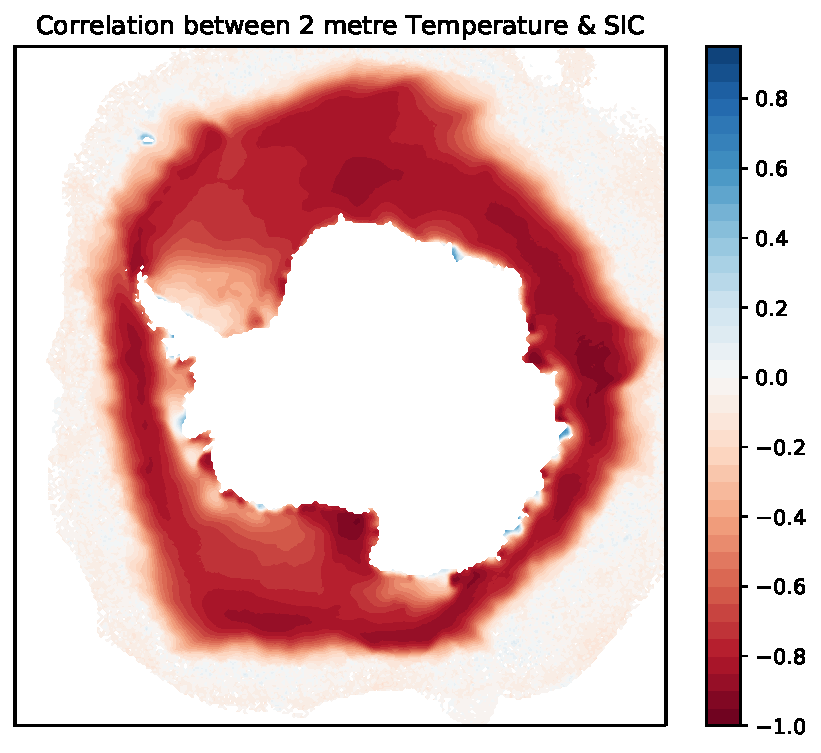
\includegraphics{Images/tempcorrwithsic.pdf}
    \caption{Correlation between temperature at 2m with sea ice concentration.}
    \label{fig:results:2mtemp_corr_with_sic}
\end{figure}

Above we have the correlation between 2 metre air temperature and sea ice concentration over Antarctica. The result that the temperature is negatively correlated with the concentration of sea ice in Antarctica is hardly surprising. Higher temperatures will be associated in the melting of ice. This both intuitively makes sense and is supported by the first law of thermodynamics (Conservation of energy). The main feature of interest in this plot is the regions which are close to the pole and there are lower correlations between 2m-temperature and SIC. It is possible that this is due to low variability in SIC in these regions over the entirety of each year.

\newpage
\section{Correlations with Sea Ice Extent}
In light of work done by other researchers which looked at global temperature correlated with the total amount of sea ice in Antarctica. \cite{Wang2019Compounding2016, Meehl2019Sustained2016} we carried out this comparison ourselves. Taking the Pearson correlation between the time series of 2m temperature at each gridpoint globally with the time series of total sea ice in Antarctica. \textcolor{red}{I'm not sure of the legitimacy of the above paragraph.}

In computing the correlations with SIE in Antarctica, we would expect the largest signal to come from seasonal variations in the different variables. This means that we are expecting large positive and negative correlations for each variable we are looking at, with spatial structures which should give us some physical understanding of how each variable acts in relation to the amount of sea ice around Antarctica.

% \begin{figure}[H]
%     \centering
%     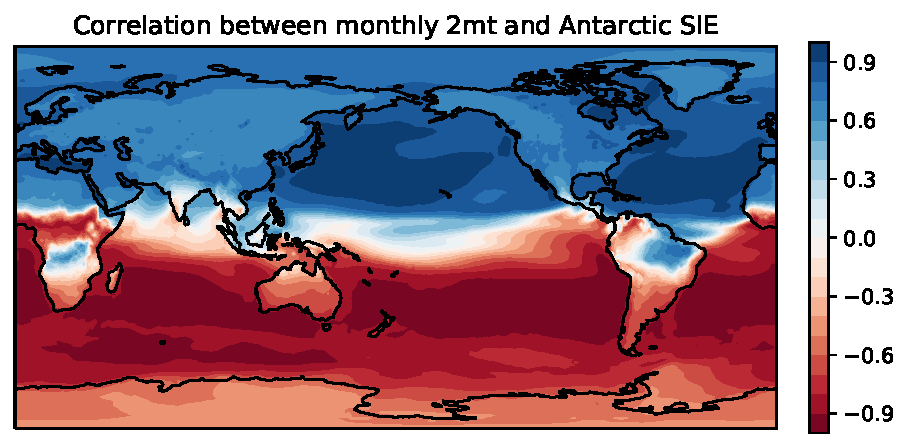
\includegraphics[width=\textwidth]{Images/global_correlation_m2mt_sie.pdf}
%     \caption{Correlation between monthly averaged 2m temperature and total SIE in Antarctica.}
%     \label{fig:my_label}
% \end{figure}

% I haven't done any preprocessing with this data so far. I believe the papers looked at some kind of anomaly in the amount of sea ice, as such I will look into doing something similar next week.
% What we see here however is good as we see a positive correlation in the northern hemisphere and a negative correlation in the southern hemisphere.

% \begin{figure}[H]
%     \centering
%     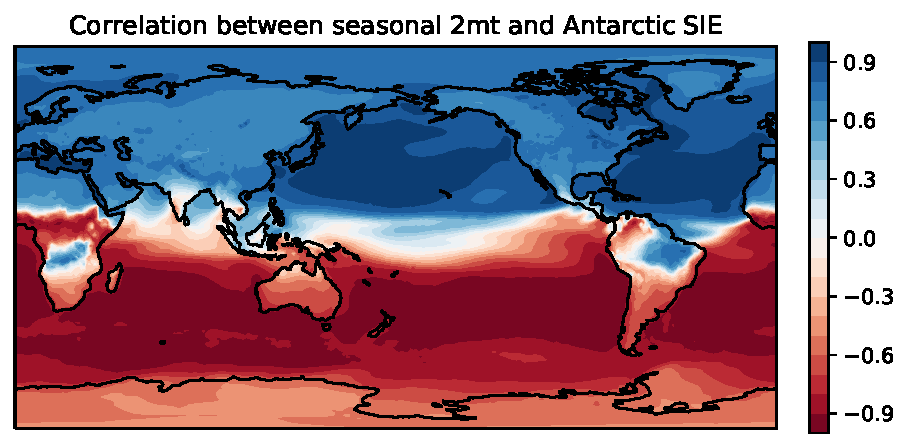
\includegraphics[width=\textwidth]{Images/global_correlation_s2mt_sie.pdf}
%     \caption{Correlation between seasonally averaged 2m temperature and total SIE in Antarctica.}
%     \label{fig:my_label}
% \end{figure}
% We note no difference between the monthly and seasonal correlations between the two datasets. This is good as we would not expect to see a large difference.


\begin{figure}[H]
    \centering
    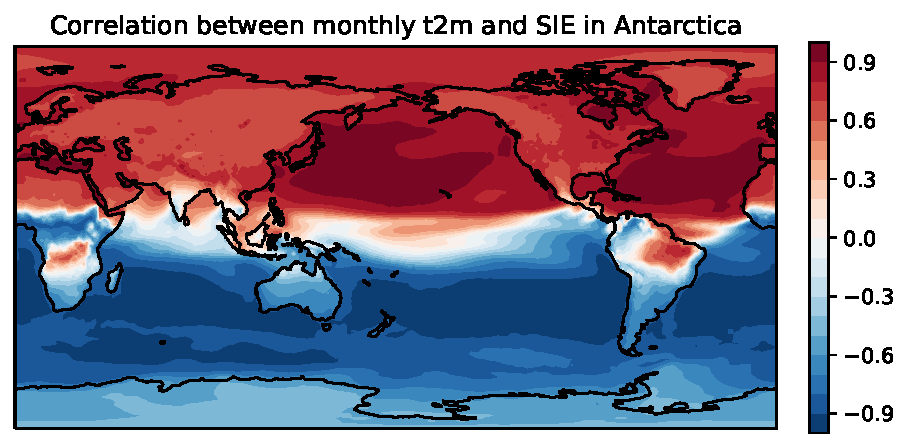
\includegraphics[width=\textwidth]{Images/global_correlation_monthly_t2m_sie.pdf}
    \caption{Correlation between 2m temperature globally and total Sea Ice Extent in Antarctica.}
    \label{fig:temp_sie_corr}
\end{figure}

We note that there is a strong seasonal signal present here. This results in the temperatures in the northern hemisphere being positively correlated with the extent of Antarctic ice. We see a corresponding negative correlation in the southern hemisphere.

We ran the same calculation also for pressure and wind speeds. The results of which are included below.
\begin{figure}[H]
    \centering
    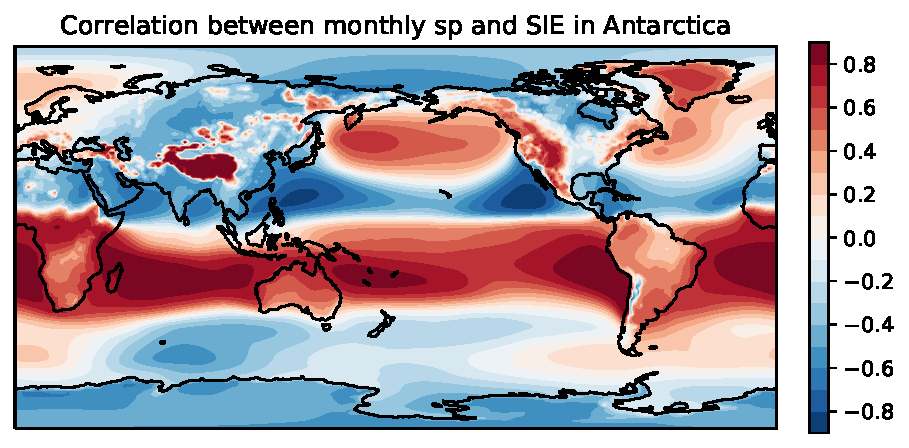
\includegraphics[width=\textwidth]{Images/global_correlation_monthly_sp_sie.pdf}
    \caption{Correlation between surface pressure globally and total Sea Ice Extent in Antarctica.}
    \label{fig:sp_sie_corr}
\end{figure}
We note that the pressure seems to be broken up longitudinally, with a negative correlation near the sea ice followed by a strong positive correlation in the tropics, another negative correlation and then a positive correlation. \textcolor{red}{Possibly because of atmospheric structure? or SAM? Explore.} Also of note is the discrepancies over land in the northern Hemisphere. \textcolor{red}{Maybe Explore?}


\begin{figure}[H]
    \centering
    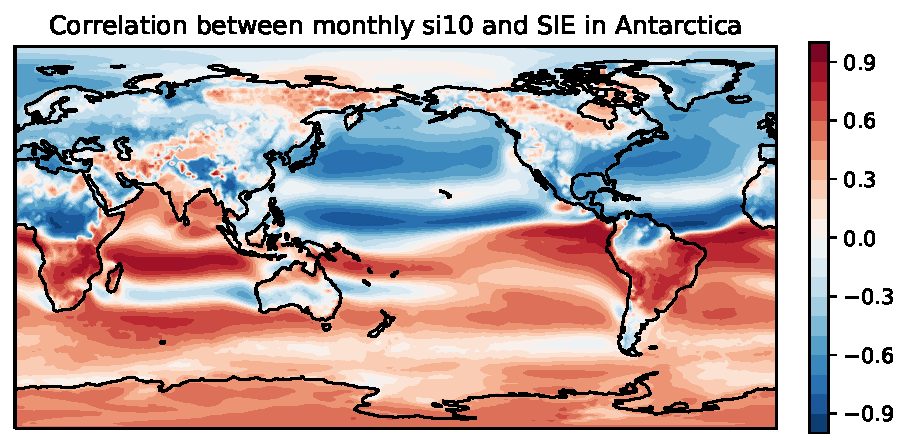
\includegraphics[width=\textwidth]{Images/global_correlation_monthly_si10_sie.pdf}
    \caption{Correlation between 10m wind speed globally and total Sea Ice Extent in Antarctica.}
    \label{fig:si10_sie_corr}
\end{figure}

The total wind speed seems generally split similarly to the temperature correlations, broken up into the northern and southern hemispheres. With generally positive correlations in the southern hemisphere and negative correlations in the northern hemisphere. This indicates potentially a strong seasonal signal which we can explore further by looking at the correlations between SIE and the u and v wind components.

\begin{figure}[H]
    \centering
    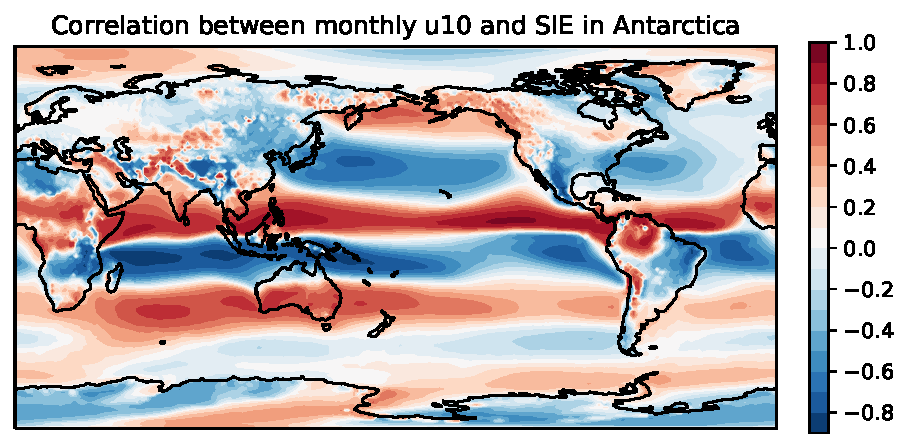
\includegraphics[width=\textwidth]{Images/global_correlation_monthly_u10_sie.pdf}
    \caption{Correlation between u component 10m wind speed globally and total Sea Ice Extent in Antarctica.}
    \label{fig:u10_sie_corr}
\end{figure}

I don't yet have a physical explanation for the bands we see here, but a structure is clearly there and worth discussing. Maybe ENSO?

\begin{figure}[H]
    \centering
    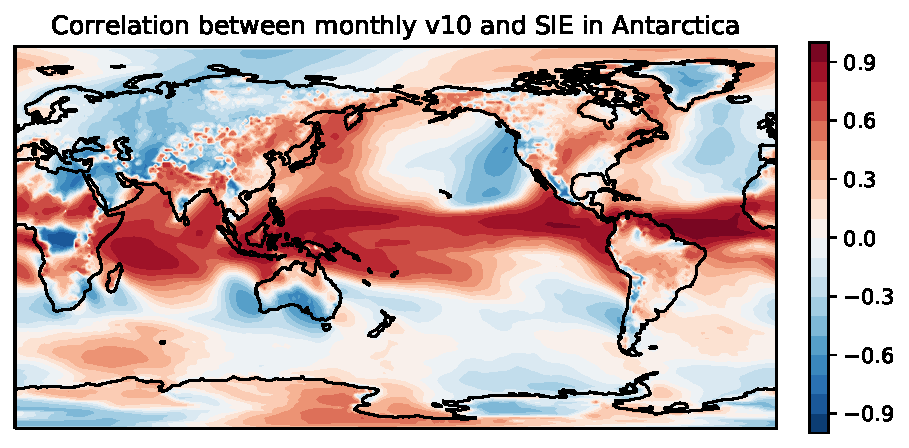
\includegraphics[width=\textwidth]{Images/global_correlation_monthly_v10_sie.pdf}
    \caption{Correlation between v component 10m wind speed globally and total Sea Ice Extent in Antarctica.}
    \label{fig:v10_sie_corr}
\end{figure}

I don't yet have a physical explanation for the bands we see here, but a structure is clearly there and worth discussing.

As expected the largest signal we are seeing in most of these plots is a seasonal one. This makes sense as the seasons are some of the largest climate drivers in the atmosphere and ocean.
\newpage
\section{Anomalous Sea Ice Extent correlations}
We are interested in more complex patterns and relations than the seasonal patterns seen in the section above. As such, we ran the same calculations as before on the anomalies for each time series we have. This was done by removing the mean value for every month from each individual value for that month over the dataset, essentially removing the seasonal component of our data. The results here are presented in the same order as the previous section, starting with 2m temperature.
% As described in the results section, we can calculate the anomaly in our data in multiple ways. For the following results we find the anomaly by removing monthly means from each location, essentially removing the interanual seasonal effect and looking at the more unrelated but perhaps more spatially complex structures in the remaining signal.
% \begin{figure}[H]
%     \begin{subfigure}[b]{\textwidth}
%          \centering
%          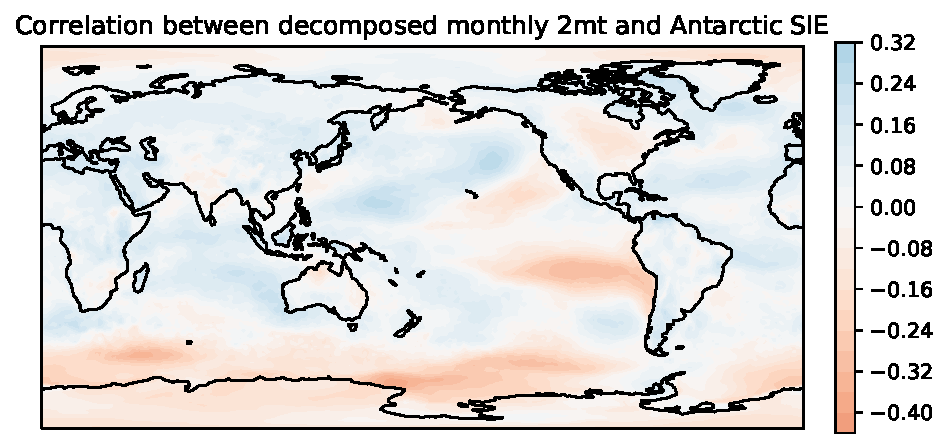
\includegraphics[width=\textwidth]{Images/global_correlation_decomposed_m2mt_sie.pdf}
%         %  \caption{Monthly decomposed 2mt correlated with antarctic SIE}
%          \label{fig:monthly_decomposed_2mt_sie}
%      \end{subfigure}
%      \begin{subfigure}[b]{\textwidth}
%          \centering
%          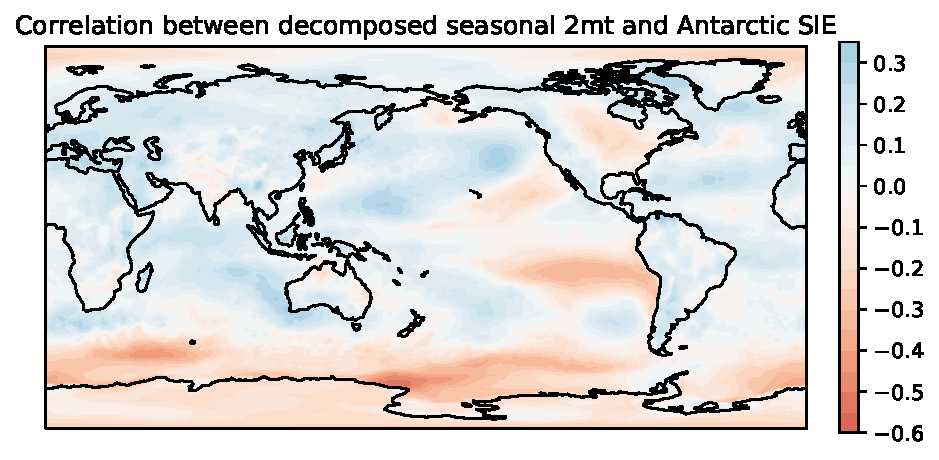
\includegraphics[width=\textwidth]{Images/global_correlation_decomposed_s2mt_sie.pdf}
%         %  \caption{Seasonal decomposed 2mt correlated with antarctic SIE}
%          \label{fig:seasonally_decomposed_2mt_sie}
%      \end{subfigure}
%     \caption{Monthly and seasonal decomposed 2mt correlated with antarctic SIE}
% \end{figure}
% We find little difference between the monthly and seasonal datasets at this point. This is good.
% Additionally, we note that the correlations are low here. This makes sense as there should be no seasonality in the data. Consequently there is also less spatial organisation in the results. The pattern vaguely reminds me of ENSO, so perhaps that is something we could look at moving forward.


\begin{figure}[H]
    \centering
    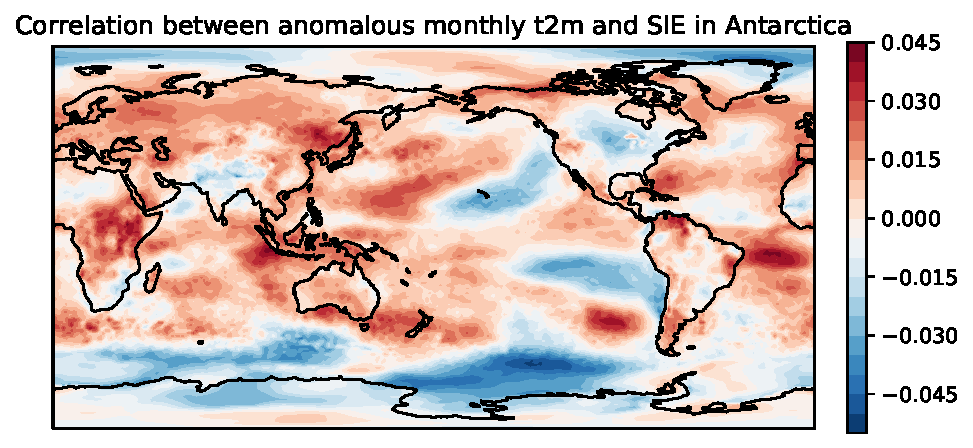
\includegraphics[width=\textwidth]{Images/global_correlation_anomalous_monthly_t2m_sie.pdf}
    \caption{Correlation between anomalous 2m temperature globally and total Sea Ice Extent in Antarctica.}
    \label{fig:t2m_anomalous_sie_corr}
\end{figure}

There is a lot to discuss about this figure, however the thing that stands out the most to me is the IPO pattern. This is something we will potentially want to look at further down the line in our calculations. Next we did the same calculation for surface pressure.

\begin{figure}[H]
    \centering
    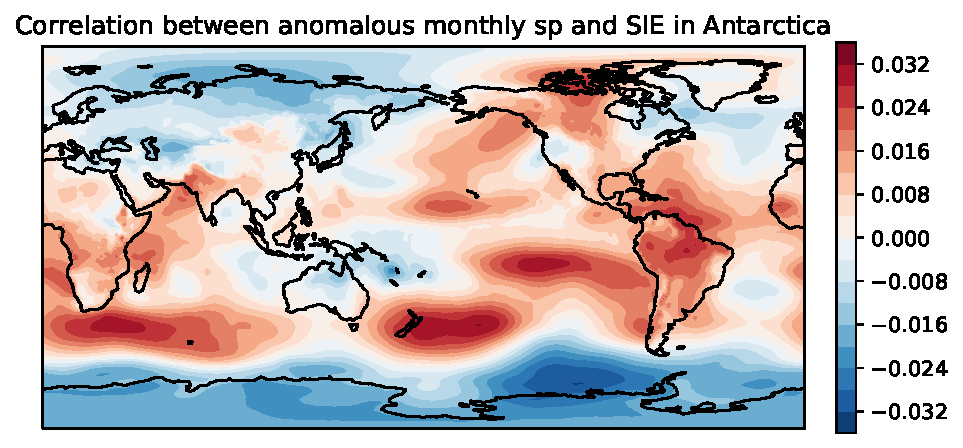
\includegraphics[width=\textwidth]{Images/global_correlation_anomalous_monthly_sp_sie.pdf}
    \caption{Correlation between anomalous surface pressure globally and total Sea Ice Extent in Antarctica.}
    \label{fig:sp_anomalous_sie_corr}
\end{figure}
The first thing to note is how large the signals are for this plot spatially. This is possibly due to how the reanalysis was done or could be showing us something deeper about our climate. I am not entirely sure at this point. Below are the results for the wind correlations.

\begin{figure}[H]
    \centering
    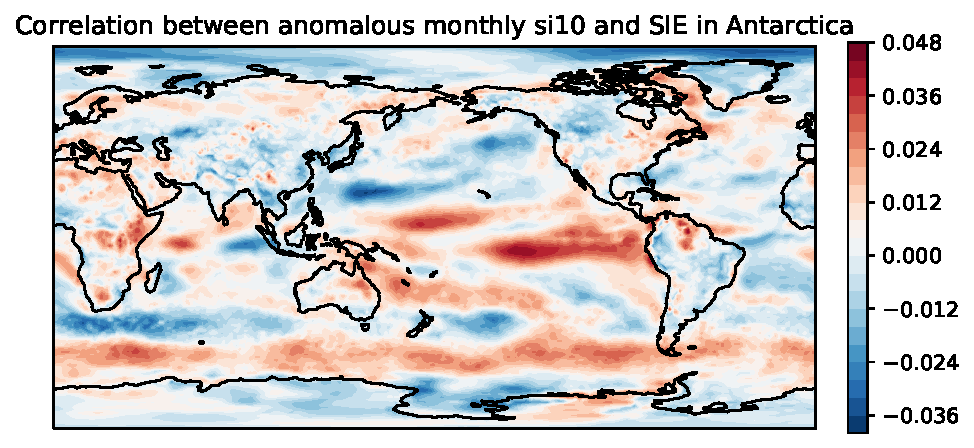
\includegraphics[width=\textwidth]{Images/global_correlation_anomalous_monthly_si10_sie.pdf}
    \caption{Correlation between anomalous 10m wind speed globally and total Sea Ice Extent in Antarctica.}
    \label{fig:si10_anomalous_sie_corr}
\end{figure}

For the total wind speed, the signal which stands out the most looks remarkably like ENSO, this is something we will want to look at further as we continue our analysis.

\begin{figure}[H]
    \centering
    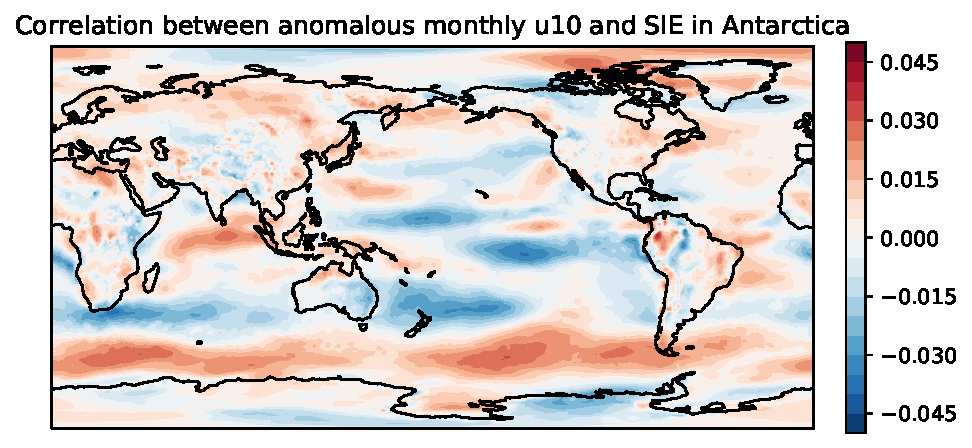
\includegraphics[width=\textwidth]{Images/global_correlation_anomalous_monthly_u10_sie.pdf}
    \caption{Correlation between anomalous u component 10m wind speed globally and total Sea Ice Extent in Antarctica.}
    \label{fig:u10_anomalous_sie_corr}
\end{figure}

For the u component wind, the signal we see could be related to ENSO but it is weaker and less spatially coherent so we cannot be totally sure.

\begin{figure}[H]
    \centering
    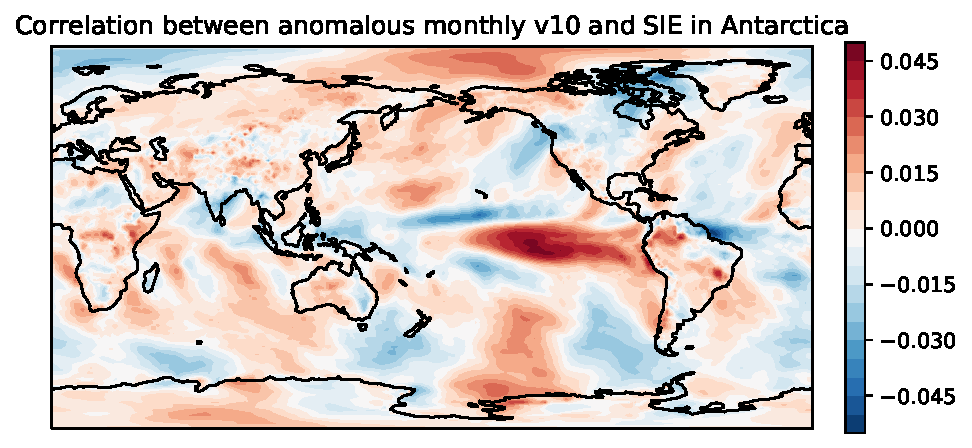
\includegraphics[width=\textwidth]{Images/global_correlation_anomalous_monthly_v10_sie.pdf}
    \caption{Correlation between anomalous v component 10m wind speed globally and total Sea Ice Extent in Antarctica.}
    \label{fig:v10_anomalous_sie_corr}
\end{figure}

For the v component of the wind we see a signal which looks remarkably like ENSO, this is something to look into further.
\newpage
\section{Mean SIC with different indicies}
\begin{table}[H]
\begin{tabular}{@{}rllll@{}}
\toprule
                                      & \textbf{SAM} & \textbf{IPO} & \textbf{DMI} & \textbf{ENSO} \\ \midrule
\textbf{raw monthly}                  & -0.0286      & -0.02356     & 0.149673     & -0.02178      \\
\textbf{raw monthly detrended}        & -0.03614     & -0.01259     & 0.14486      & -0.02917      \\
\textbf{anomalous monthly}            & \textbf{0.153142}     & \textbf{-0.12784}     & 0.112879     & 0.067515      \\
\textbf{anomalous monthly detrended}  & \textbf{0.117848}     & -0.06747     & 0.113995     & 0.02886       \\
\textbf{raw seasonal}                 & -0.04518     & -0.0298      & 0.05791      & -0.01521      \\
\textbf{raw seasonal detrended}       & -0.06096     & -0.0148      & 0.055534     & -0.02615      \\
\textbf{anomalous seasonal}           & \textbf{0.191653}     & -0.14036     & 0.026778     & 0.092851      \\
\textbf{anomalous seasonal detrended} & 0.131356     & -0.06952     & 0.006859     & 0.043756      \\
\textbf{raw annual}                   & 0.270046     & -0.13599     & 0.014287     & 0.115359      \\
\textbf{raw annual detrended}         & 0.13903      & -0.02698     & -0.02919     & 0.028031      \\
\textbf{anomalous annual}             & 0.278939     & -0.16029     & 0.014941     & 0.135027      \\
\textbf{anomalous annual detrended}   & 0.144474     & -0.05059     & -0.03012     & 0.046729      \\ \bottomrule
\end{tabular}
\caption{Correlations between different indices and SIC in Antarctica. Bold values indicate statistical significance i.e. a p-value lower than 0.05.}
\end{table}

% Please add the following required packages to your document preamble:
% \usepackage{booktabs}
\begin{table}[H]
\begin{tabular}{@{}rllll@{}}
\toprule
                                      & \textbf{SAM} & \textbf{IPO} & \textbf{DMI} & \textbf{ENSO} \\ \midrule
\textbf{raw monthly}                  & 0.53     & 0.60     & 0.24     & 0.63      \\
\textbf{raw monthly detrended}        & 0.43     & 0.78     & 0.25     & 0.52      \\
\textbf{anomalous monthly}            & 0.00     & 0.00     & 0.37     & 0.14      \\
\textbf{anomalous monthly detrended}  & 0.00     & 0.14     & 0.37     & 0.52      \\
\textbf{raw seasonal}                 & 0.57     & 0.70     & 0.48     & 0.84      \\
\textbf{raw seasonal detrended}       & 0.44     & 0.85     & 0.50     & 0.74      \\
\textbf{anomalous seasonal}           & 0.01     & 0.07     & 0.74     & 0.24      \\
\textbf{anomalous seasonal detrended} & 0.09     & 0.38     & 0.93     & 0.58      \\
\textbf{raw annual}                   & 0.09     & 0.40     & 0.93     & 0.47      \\
\textbf{raw annual detrended}         & 0.39     & 0.86     & 0.86     & 0.86      \\
\textbf{anomalous annual}             & 0.08     & 0.32     & 0.92     & 0.40      \\
\textbf{anomalous annual detrended}   & 0.37     & 0.75     & 0.85     & 0.77      \\ \bottomrule
\end{tabular}
\caption{p-values for the above correlations.}
\end{table}

\section{Annually averaged results}
For the annually averaged time series, no time-shift was included and there is no difference between the raw and anomalous datasets so we only have two plots, one with the trend and one without.
\begin{figure}[H]
    \centering
    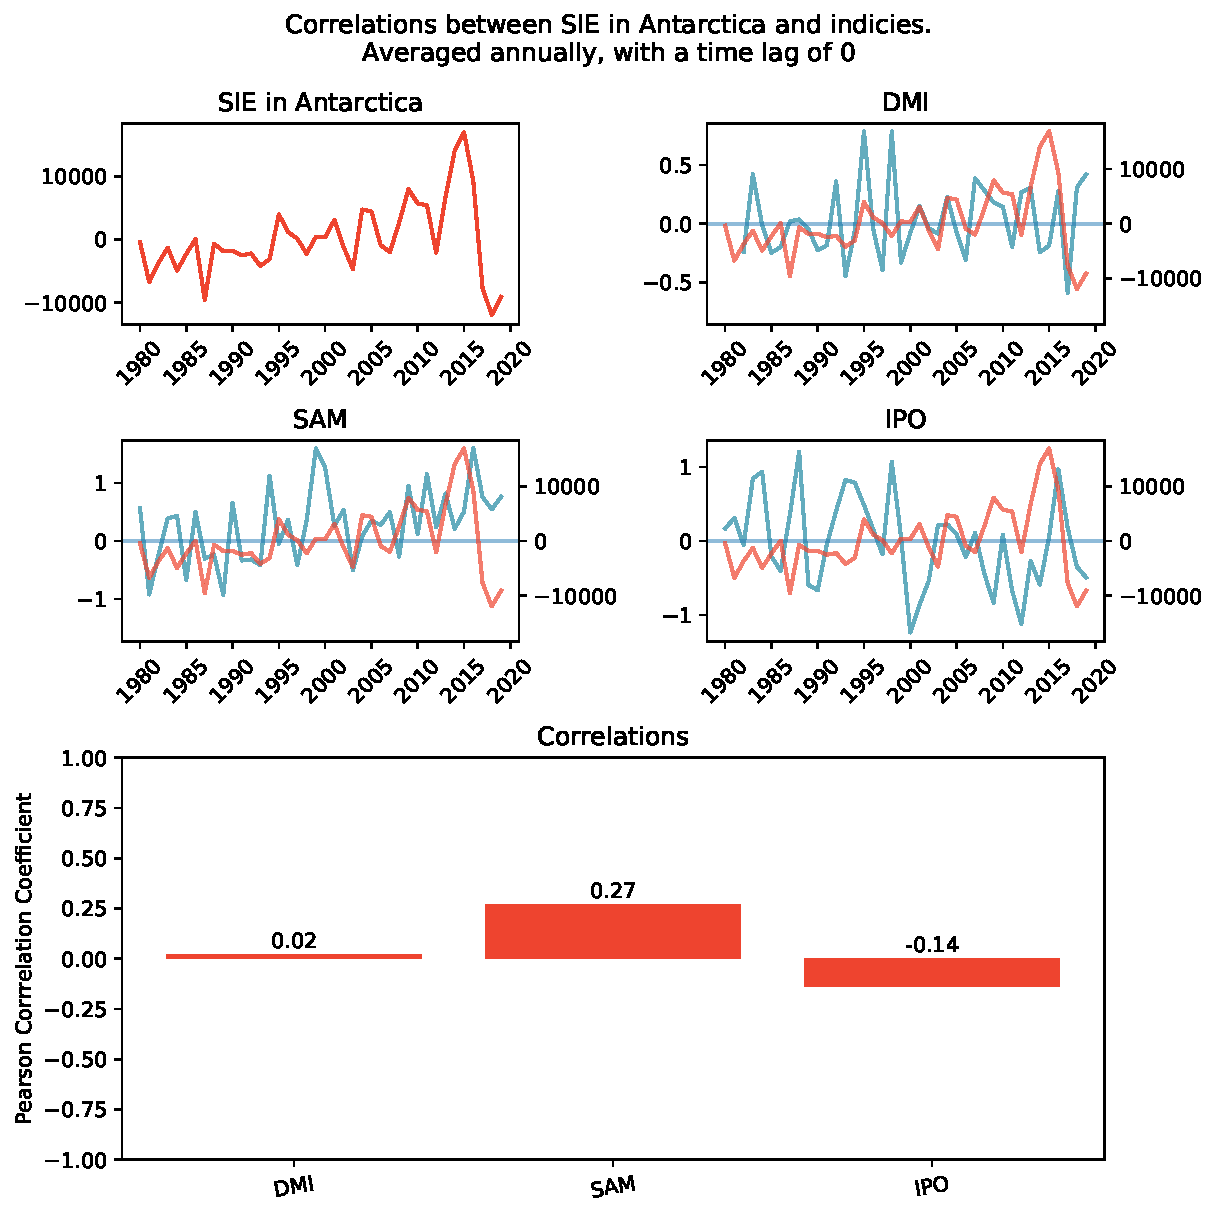
\includegraphics[width=\linewidth]{Images_3.0/correlations/subplots_indicies_annually_0_anomalous.pdf}
    \caption[Correlations between SIE in Antarctica and indices, averaged annually with no time lag.]{Correlations between SIE in Antarctica and indices, averaged annually with no time lag. The first 4 plots are time series of total SIE and the different indices so we can visually gain an understanding regarding the correlations. The bottom plot is a bar plot showing the correlations between SIE and the different indices. Blue bars have a p-value less than 0.05 and are considered statistically significant. Red bars have a p-value larger than 0.05 and are considered statistically insignificant.}
    \label{fig:anual_with_trend}
\end{figure}

\begin{figure}[H]
    \centering
    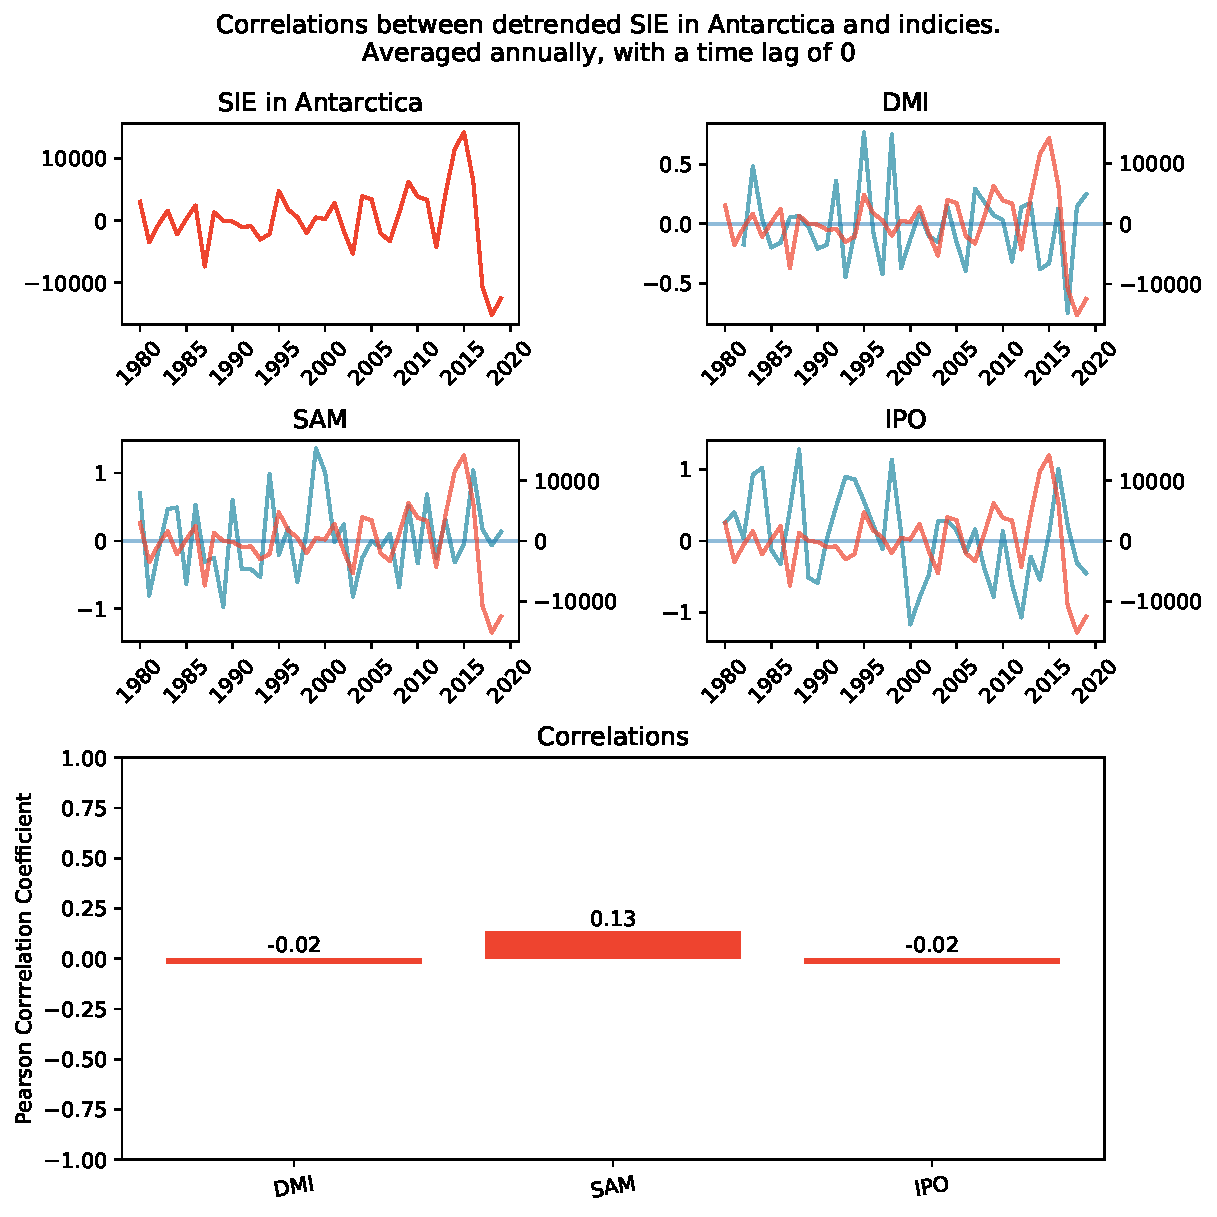
\includegraphics[width=\linewidth]{Images_3.0/correlations/subplots_indicies_annually_0_anomalous_detrended.pdf}
    \caption[Correlations between SIE in Antarctica and indices, averaged annually and detrended with no time lag.]{Correlations between SIE in Antarctica and indices, averaged annually and detrended with no time lag. The first 4 plots are time series of total SIE and the different indices so we can visually gain an understanding regarding the correlations. The bottom plot is a bar plot showing the correlations between SIE and the different indices. Blue bars have a p-value less than 0.05 and are considered statistically significant. Red bars have a p-value larger than 0.05 and are considered statistically insignificant.}
    \label{fig:annual_without_trend}
\end{figure}
Not much can be said from the above figures as all the correlations are insignificant. This could be for a number of reasons, not least because we are only looking at 40 data-points for each time series or that we are considering the behaviour of ice over a large spatial area. Though still statistically insignificant, the correlations are larger for the case where the trend is included.


\section{Monthly averages}

In order to hopefully gain better results, we looked at this with a higher temporal resolution (monthly rather than annually averaged). This has the advantage of picking up higher frequency behaviours, but also is more noisy as a result. Additionally with the higher resolution it makes sense to explore lead-lag relationships between the different variables, this is something we do later in this thesis.


\begin{figure}[H]
    \centering
    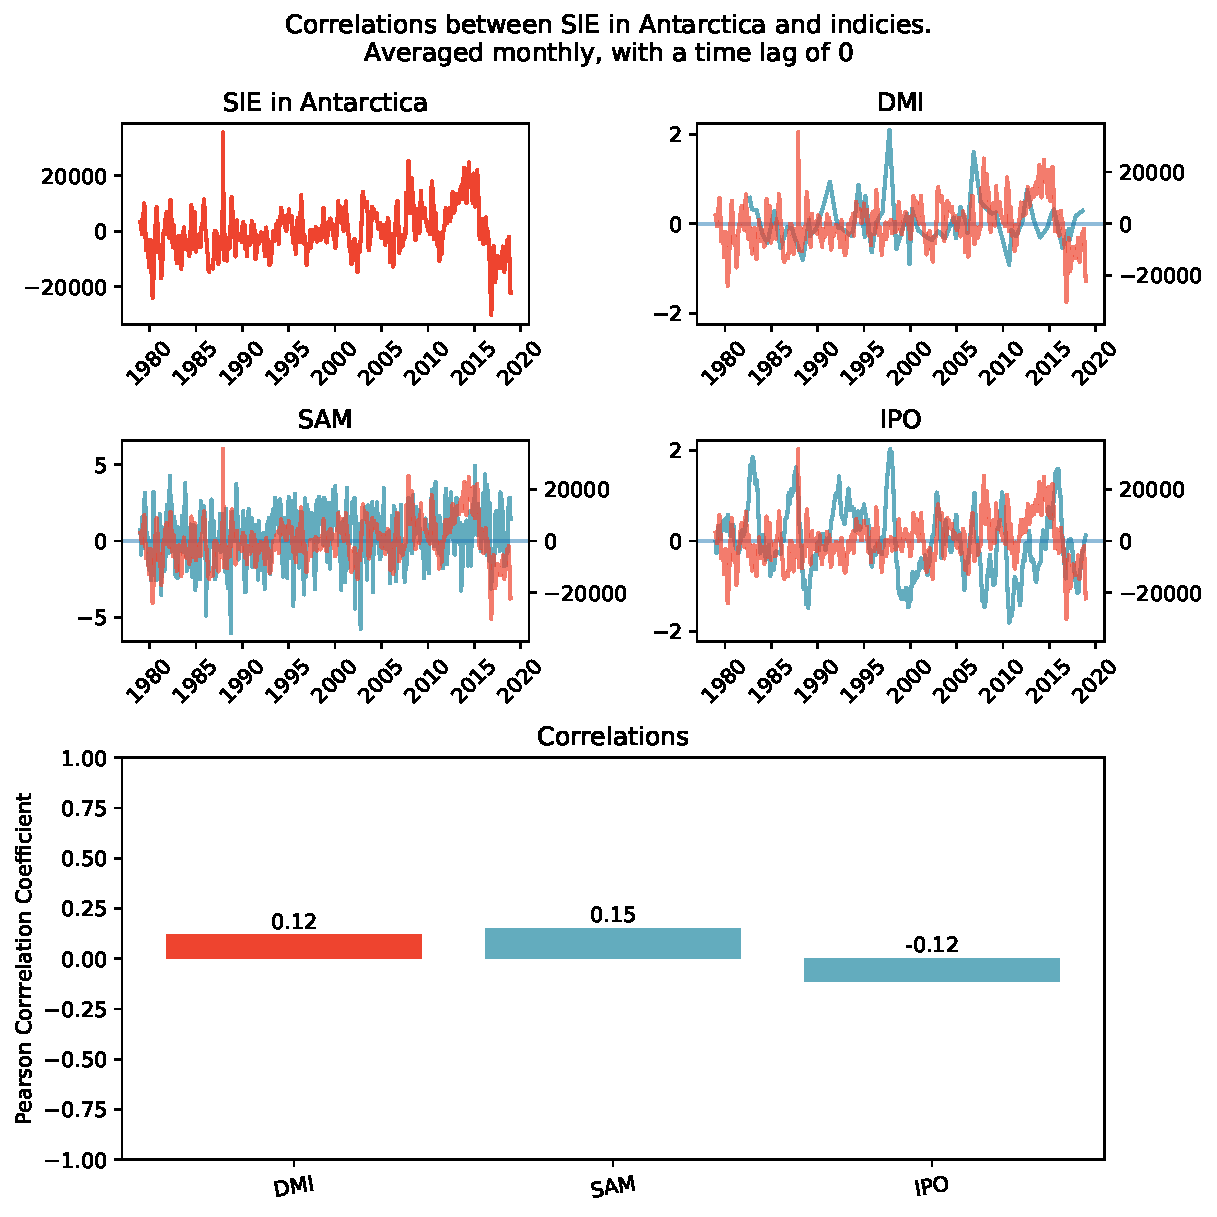
\includegraphics[width = \linewidth]{Images_3.0/correlations/subplots_indicies_monthly_0_anomalous.pdf}
    \caption[Correlations between SIE in Antarctica and indices, averaged monthly with no time lag.]{Correlations between SIE in Antarctica and indices, averaged monthly with no time lag. The first 4 plots are time series of total SIE and the different indices so we can visually gain an understanding regarding the correlations. The bottom plot is a bar plot showing the correlations between SIE and the different indices. Blue bars have a p-value less than 0.05 and are considered statistically significant. Red bars have a p-value larger than 0.05 and are considered statistically insignificant.}
    \label{fig:seasonal_with_trend}
\end{figure}
Immediately, this figure tells us that SAM and IPO both have significant correlations with SIE in Antarctica on a monthly basis. For SAM this is unsurprising as the pattern is defined as changes in wind speeds and pressures at the high southern latitudes close to Antarctica \textcolor{red}{(get proper definition and cite}. For IPO this is also makes some sense as it is a major climate signal over the Pacific. \textcolor{red}{Do other people get the same result?} To help build our understanding of these relationships, let's look at what happens when we detrend the time series.

\begin{figure}[H]
    \centering
    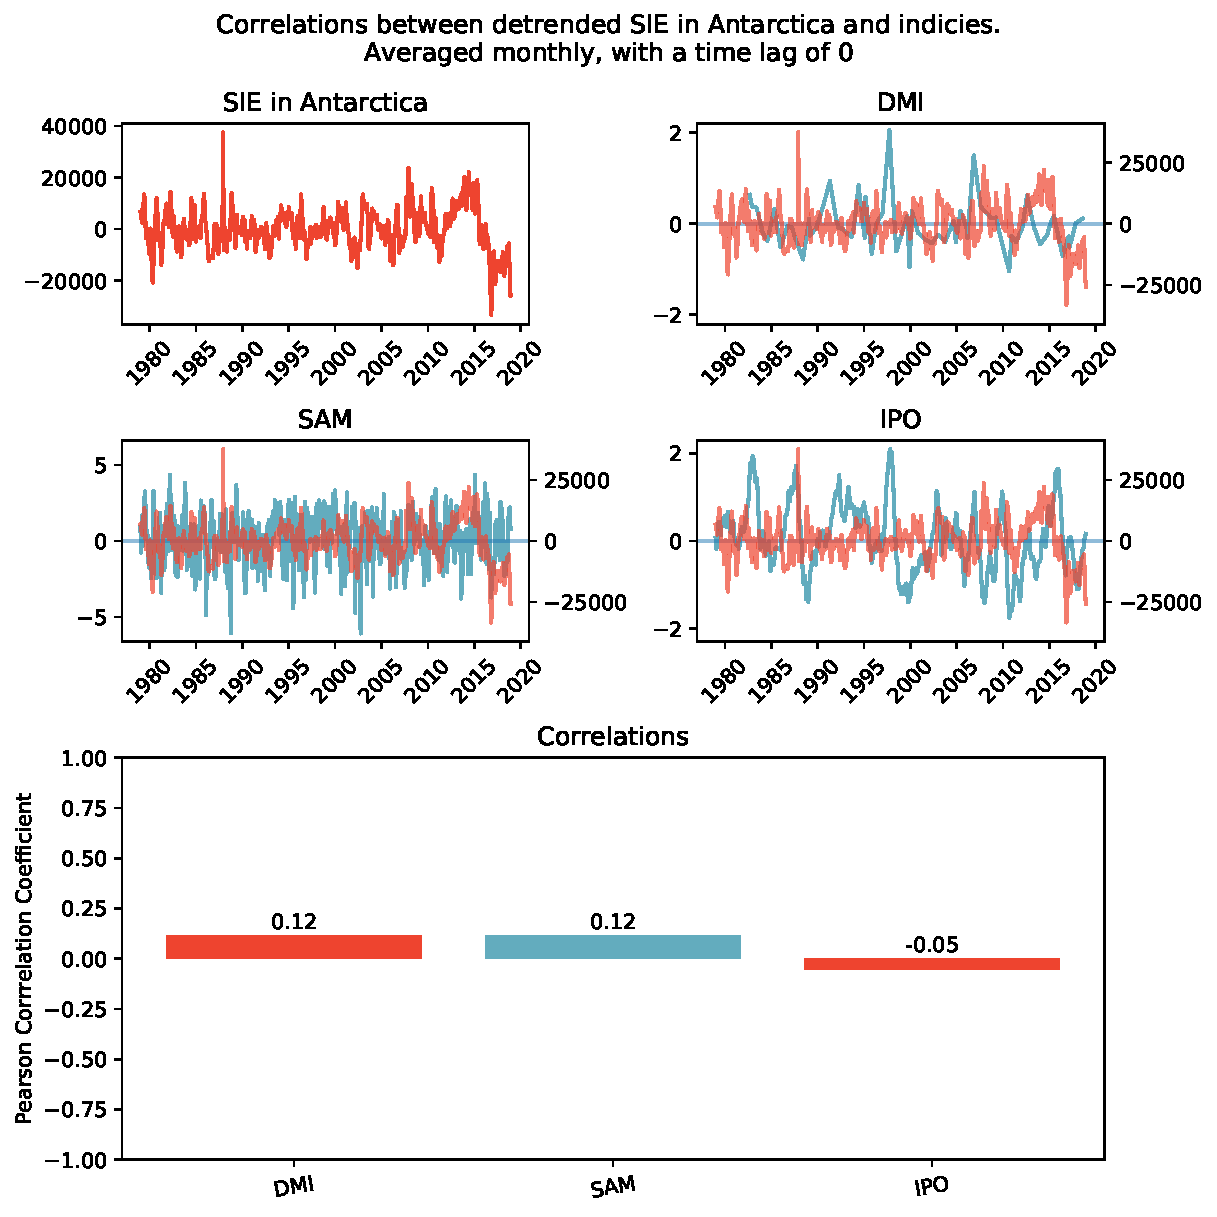
\includegraphics[width = \linewidth]{Images_3.0/correlations/subplots_indicies_monthly_0_anomalous_detrended.pdf}
    \caption[Correlations between SIE in Antarctica and indices, averaged monthly, detrended with no time lag.]{Correlations between SIE in Antarctica and indices, averaged monthly, detrended with no time lag. The first 4 plots are time series of total SIE and the different indices so we can visually gain an understanding regarding the correlations. The bottom plot is a bar plot showing the correlations between SIE and the different indices. Blue bars have a p-value less than 0.05 and are considered statistically significant. Red bars have a p-value larger than 0.05 and are considered statistically insignificant.}
    \label{fig:seasonal_without_trend}
\end{figure}

When we remove the trend the magnitude of the correlations decrease for SAM and IPO, whereas DMI has no change in the magnitude of correlation. The correlation between SAM and SIE in Antarctica remains statistically significant whereas the IPO is no longer significant. 


\section{Lead lag analysis for monthly data}

We can perform some lead-lag analysis on the correlations between the different indices and SIE in Antarctica, to gain some understanding on if there are any delayed signals of significance we need to consider. Because the indices are initially anomalous signals, we only did this for the anomalous sea ice data. In the following plots, a negative time-lag indicates that we are comparing the time-series for sea ice with patterns in each index before that point. A positive time-lag indicates that we are comparing the time-series for sea ice with patterns in each index after that point. The size of the time-lag indicates the length to which the sea ice time series was shifted.
\begin{figure}[H]
    \centering
    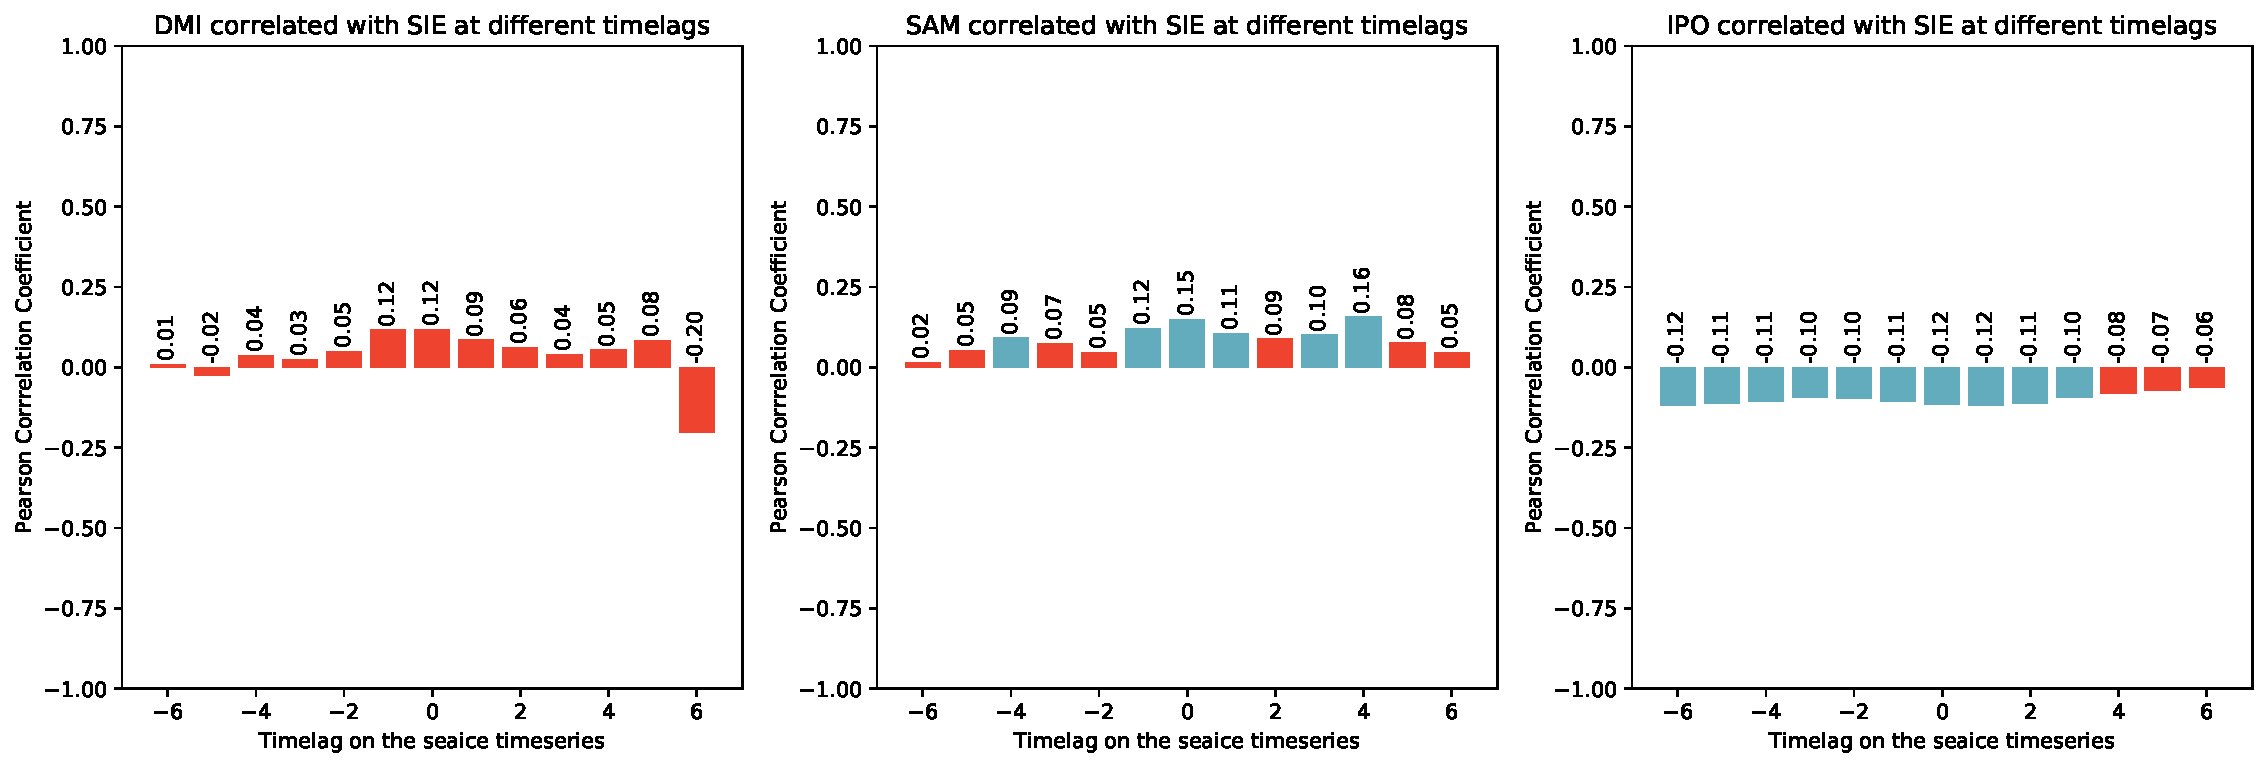
\includegraphics[width = \linewidth]{Images_3.0/correlations/indicies_monthly_anomalous.pdf}
    \caption[Histograms of correlations with different indices at different time-lags with anomalous Antarctic SIE.]{Histograms of correlations with different indices at different time-lags with anomalous Antarctic SIE. A blue bar indicates a statistically significant p-value of less than 0.05. A red bar indicates a statistically insignificant value.}
    \label{fig:leadlag_anomalous}
\end{figure}

DMI has no significant correlation with Antarctic SIE regardless of time-lag. SAM has a significant correlation for time-lags of -1, 0, 1, 3, 4, and 5 months. IPO has significant correlations for any time-lag less than 3 months (including negative time-lags). It's possible that the trend is confusing the signals here so let's see what happens when we remove it.

\begin{figure}[H]
    \centering
    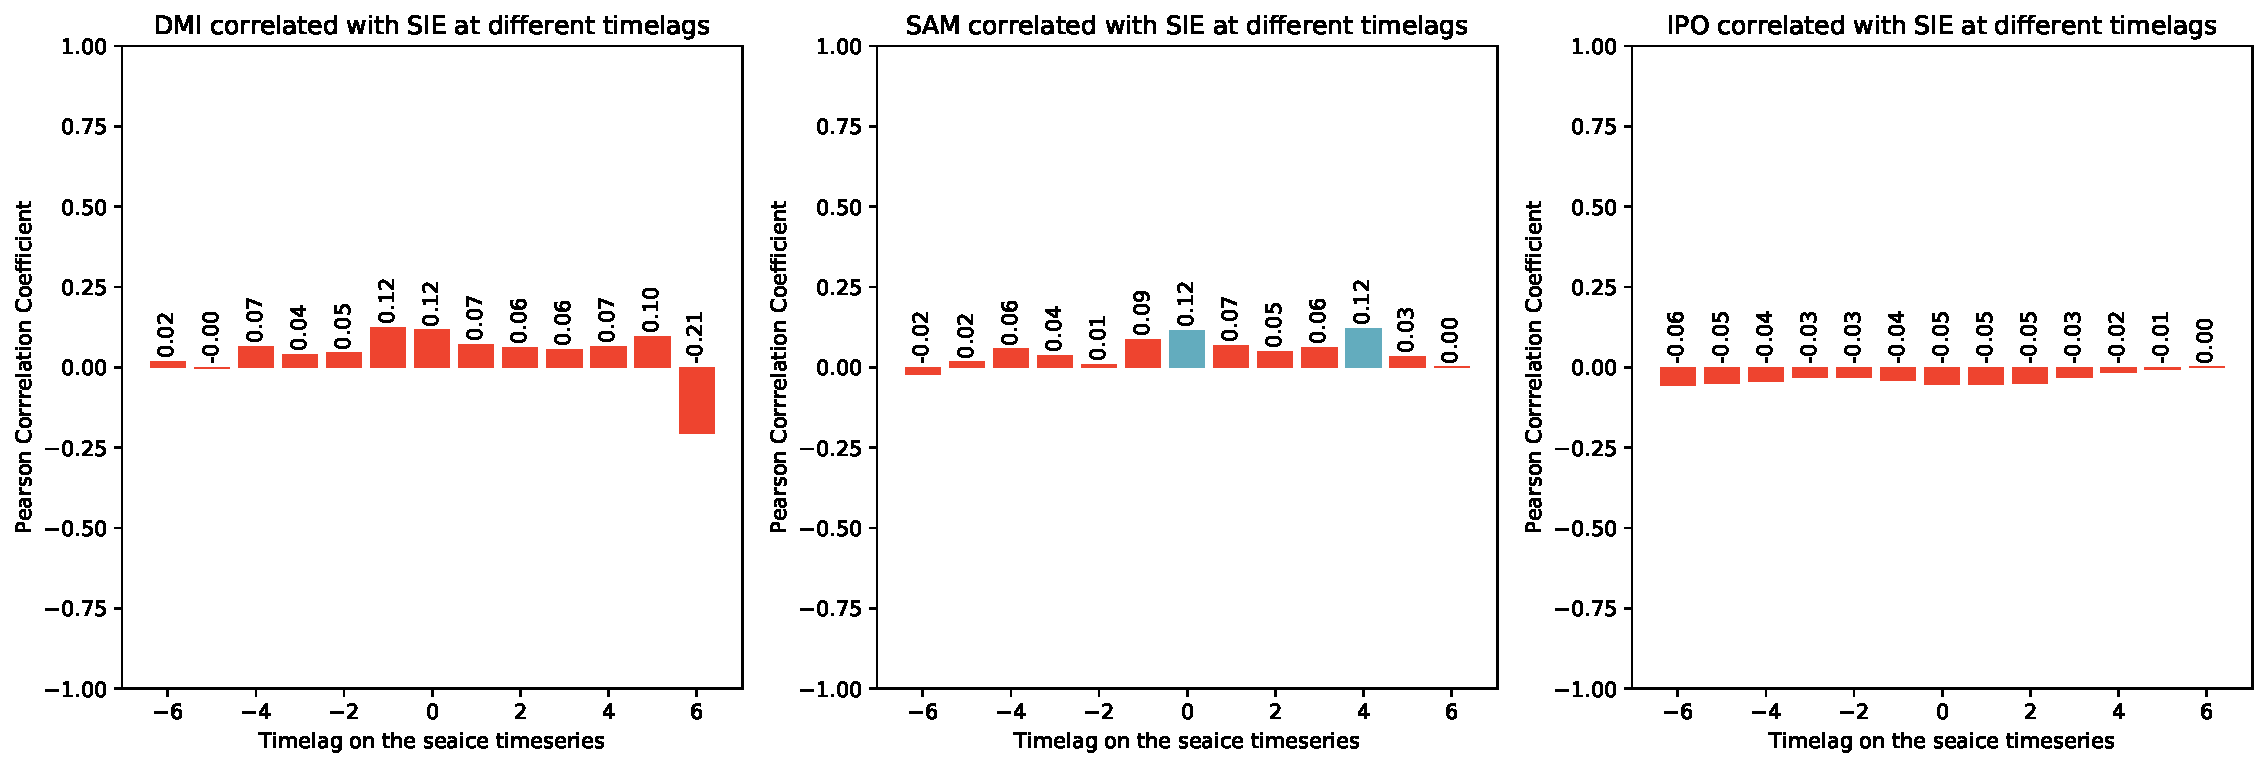
\includegraphics[width = \linewidth]{Images_3.0/correlations/indicies_monthly_anomalous_detrended.pdf}
    \caption[Histograms of correlations with different indices at different time-lags with anomalous and detrended Antarctic SIE.]{Histograms of correlations with different indices at different time-lags with anomalous and detrended Antarctic SIE. A blue bar indicates a statistically significant p-value of less than 0.05. A red bar indicates a statistically insignificant value.}
    \label{fig:leadlag_anomalous_detrended}
\end{figure}

The only significant correlations we observe at this point are the correlations between SAM and Antarctic SIE for time-lags of 0 and 4 months. This indicates that when an event occurs for Antarctic SIE, it is likely that we would observe a related event in the SAM index at the same time and also 4 months later. \textcolor{red}{not sure if I worded this right so let's go with it for now.}\medskip

One problem we have here is that we are not totally able to use the information for the correlations which we have above to inform us regarding how events for the different indexed circulations could potentially impact the behaviour of sea ice we see in Antarctica. For that we want to look at the first time derivative of Antarctic SIE to see if it has behaviours related to these indices.
\newpage
\section{Splitting the data}
Throughout literature surrounding the behaviour of Antarctic SIE, there is a large focus on the overall increase in SIE up to 2014, \cite{Parkinson2019} for instance spends some time discussing this, as does \cite{Yuan2017}. They also go into some detail of the spatial variability. More focus is also put on the large decrease in the SIE from 2014 where we get the record largest amount of SIE to 2016 when we get the record lowest SIE. \cite{Meehl2018}
\newpage
\section{Spatial distributions of correlations}
Considering the correlations between the different variables, we can look at the spatial distribution of Antarctic SIE with the different indices. Starting with the raw data from each grid point correlated with the different indices we get the following figure. We note that most of the correlations here are weak and insignificant. This is probably due to the seasonal cycle being the dominating factor in the time series before anything else is done.
\begin{figure}[H]
    \centering
    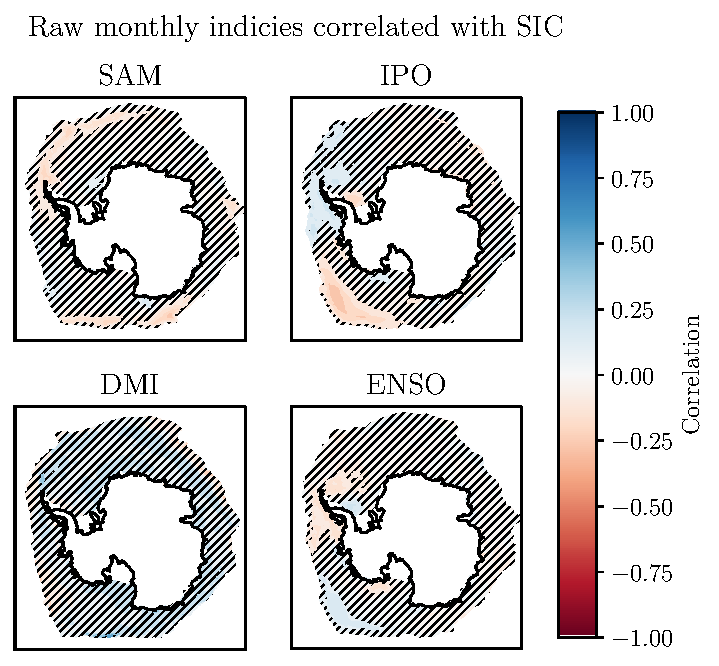
\includegraphics{images_v2/correlations/spatial/raw_monthly_raw_1_nsidc.pdf}
    \caption[Raw monthly indices correlated with SIE at individual gridpoints around Antarctica.]{Raw monthly indices correlated with SIE at individual gridpoints around Antarctica from the NSIDC dataset. Blue indicates a positive correlation and red indicates a negative correlation. Regions with a p-value larger than 0.05 has been hashed out. The unhatched regions are statistically significant.}
    \label{fig:my_label}
\end{figure}

The results above make sense but do not tell us a lot, other than highlighting that the western side of Antarctica seems to be more significantly related to the different indices. This may be due to the geography of the Antarctic peninsula.
\newpage


\chapter{Regressions}

Following on from the correlation results shown before it is apparent that there are potential relationships between the different atmospheric circulations and the behaviour in trends and variability of sea ice extent in Antarctica. The next step is to begin to quantify the extent of this relationship by performing a regression analysis. The mechanics of how these figures are produced are described in detail in the method section \textcolor{red}{cross-reference this}. 

For this section we will start by looking at the mean SIE across the entire continent and fit it to a simple linear model which predicts a value of SIE from the values of the different circulations we are looking at. To begin with this is SAM, DMI and IPO, however as our analysis expands, we plan to look at other influential circulations such as ENSO.

Following this we will perform the same analysis on each gridpoint of sea-ice and look at the spatial distribution of this regression. Using it to quantify and investigate the extent to which we can account for variability in SIE to these different indices.

What we are expecting to see is that SAM will have the largest impact on long term trends and DMI and IPO will be more important for describing short term variability.

\newpage
\section{Regression analysis on mean annual SIE}

Before doing any spatial analysis we will take a moment to apply the regression analysis to the mean value of SIE over our time period. The simplest and first step we take is to plot the annual values of SIE against each of the indices we are investigating.
\begin{figure}[H]
    \centering
    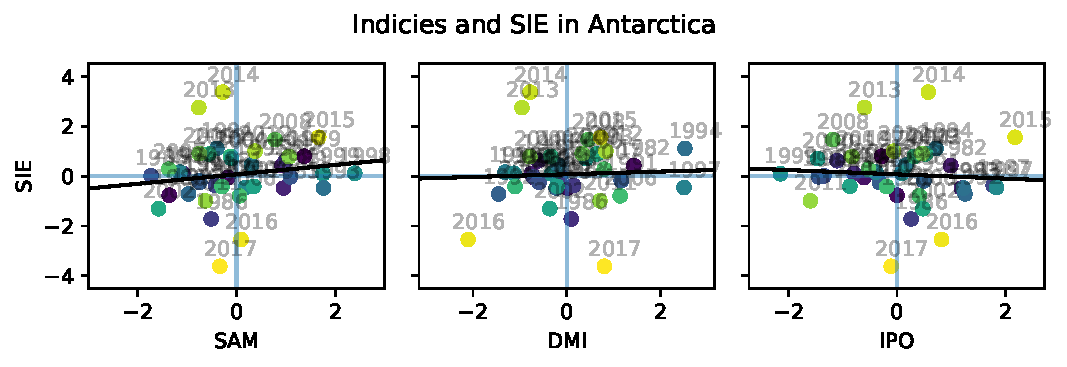
\includegraphics[width=\linewidth]{Images_3.0/regressions/scatter_anomalous_n1_annually_detrended_1979_2018.pdf}
    \caption{Regression of SIC for each of the indices for 1979 to 2018.}
    \label{fig:scatter_anomalous_n1_annually_1979_2018}
\end{figure}
We note that these results are consistent with what we found in the correlation analysis. SAM has a positive relationship with SIE, while DMI has a very weak positive relationship and IPO has a weak negative relationship. This doesn't give us new information, however the consistency indicates that the regression analysis provides somewhat reliable results results. Plotting the same thing for before and after December 2001 when IPO is in negative and positive phases respectively gives the following plots.

\begin{figure}[H]
    \begin{subfigure}{\linewidth}
    \centering
    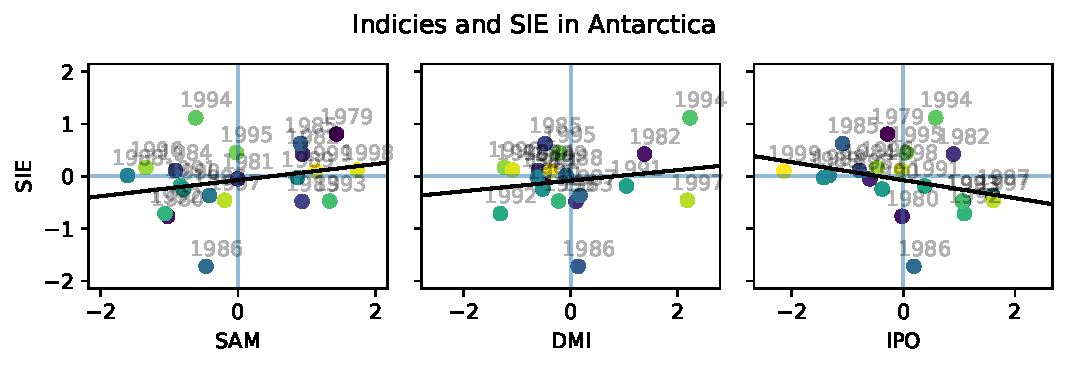
\includegraphics[width=\linewidth]{Images_3.0/regressions/scatter_anomalous_n1_annually_detrended_1979_2000.pdf}
    \caption{Regression of SIC for each of the indices for 1979 to 2000.}
    \label{fig:scatter_anomalous_n1_annually_1979_2000}
    \end{subfigure}
    
    \begin{subfigure}{\linewidth}
    \centering
    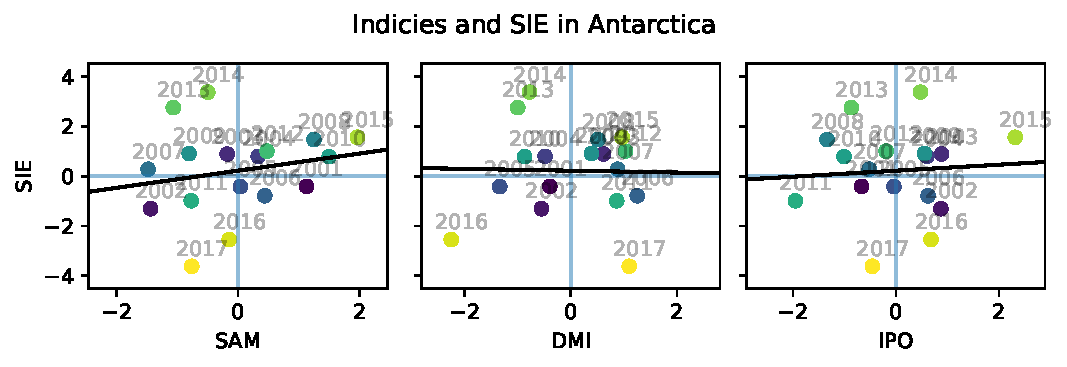
\includegraphics[width=\linewidth]{Images_3.0/regressions/scatter_anomalous_n1_annually_detrended_2001_2018.pdf}
    \caption{Regression of SIC for each of the indices for 2001 to 2018.}
    \label{fig:scatter_anomalous_n1_annually_2001_2018}
    \end{subfigure}
    \caption{Regressions for SIE for the different time periods in our dataset.}
\end{figure}
Here we can see that there is little change for the SAM relationship with SIE whereas the relationship between IPO experiences a significant change, shifting from a negative relationship before 2001 and a positive relationship after 2001. DMI has a positive relationship before 2001 and a weak negative relationship after 2001.

\subsection{Regression analysis on mean monthly SIE}
We have the same plots for the monthly version of the data.
\begin{figure}[H]
    \begin{subfigure}{\linewidth}
    \centering
    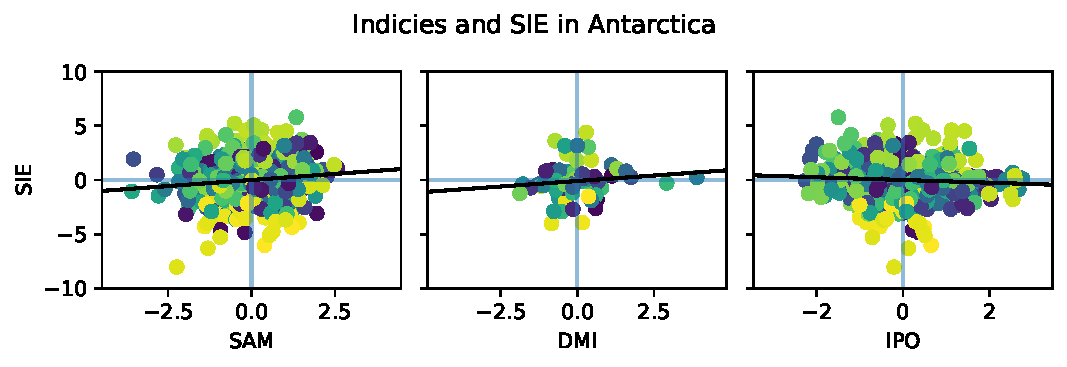
\includegraphics[width=\linewidth]{Images_3.0/regressions/scatter_anomalous_n1_monthly_detrended_1979_2018.pdf}
    \caption{Regression of SIC for each of the indices for 1979 to 2018.}
    \label{fig:scatter_anomalous_n1_annually_1979_2018}
    \end{subfigure}
    
    \begin{subfigure}{\linewidth}
    \centering
    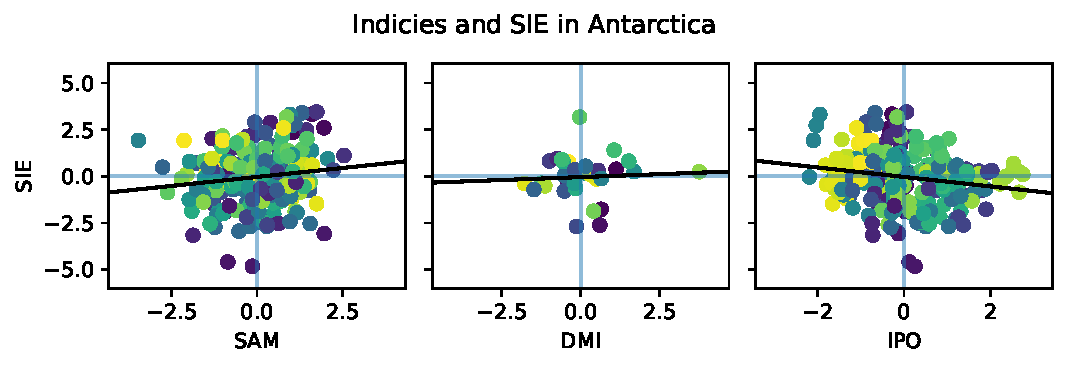
\includegraphics[width=\linewidth]{Images_3.0/regressions/scatter_anomalous_n1_monthly_detrended_1979_2000.pdf}
    \caption{Regression of SIC for each of the indices for 1979 to 2000.}
    \label{fig:scatter_anomalous_n1_annually_1979_2000}
    \end{subfigure}
    
    \begin{subfigure}{\linewidth}
    \centering
    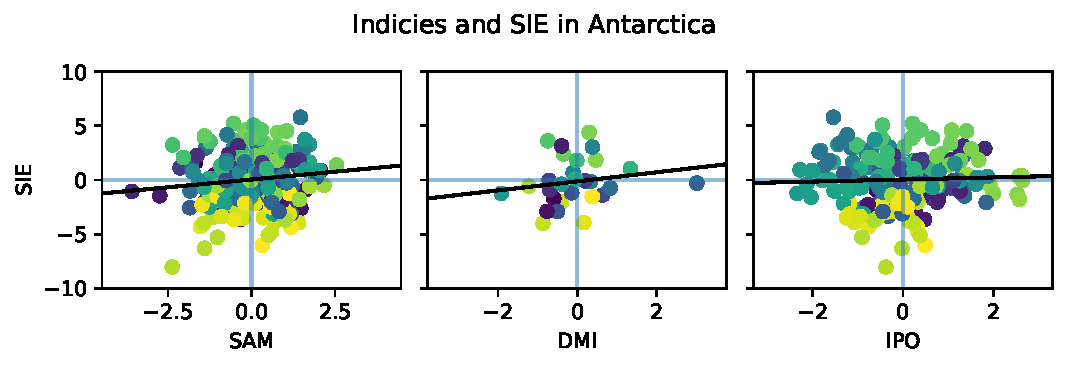
\includegraphics[width=\linewidth]{Images_3.0/regressions/scatter_anomalous_n1_monthly_detrended_2001_2018.pdf}
    \caption{Regression of SIC for each of the indices for 2001 to 2018.}
    \label{fig:scatter_anomalous_n1_annually_2001_2018}
    \end{subfigure}
    \caption[Regressions for SIE for the different time periods in our dataset.]{Regressions for SIE for the different time periods in our dataset. The colour represents years with blue being early years and yellow representing latter years.}
\end{figure}
The main difference in these plots when compared with the annual averages is the relationship between SIE and IPO and DMI after 2001. DMI has a positive relationship for the monthly means whereas it has a negative relationship for the annual means. IPO has a weaker relationship for the monthly means than the annual means.
\section{Applying the regression model}
After doing this initial analysis we can apply the regression analysis using the model:
$$
\text{SIE} = a\times\text{SAM} + b\times\text{DMI} + c \times\text{IPO} + d
$$
We can look at the quality of this fit by plotting this model prediction and the actual SIE time-series against each other.
\begin{figure}[H]
    % \begin{subfigure}{\linewidth}
    \centering
    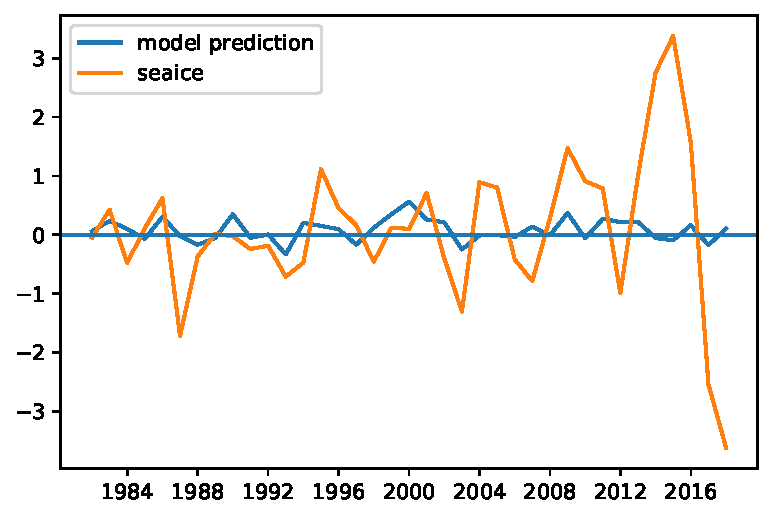
\includegraphics{Images_3.0/regressions/multivariate_model_anomalous_n1_annually_detrended_1979_2018.pdf}
    \caption{Fitted model for SIE detrended and averaged annually from 1979 to 2018.}
    \label{fig:multivariate_model_anomalous_n1_annually_detrended_1979_2018}
    % \end{subfigure}
\end{figure}
This doesn't seem to be a good fitting. This isn't surprising for a number of reasons. Firstly the regressions done on each individual index were each relatively weak and so we don't expect a strong fitting when done in concert. Additionally the system we are looking at is intrinsically complex and probably nonlinear, which leads to a bad fitting with a linear model. Additionally because we are only looking at the mean value for SIE this plot will have lost information because the indices probably affect different spatial regions of SIC in different ways. This is something we will explore further.
\begin{figure}[H]
    \begin{subfigure}{\linewidth}
    \centering
    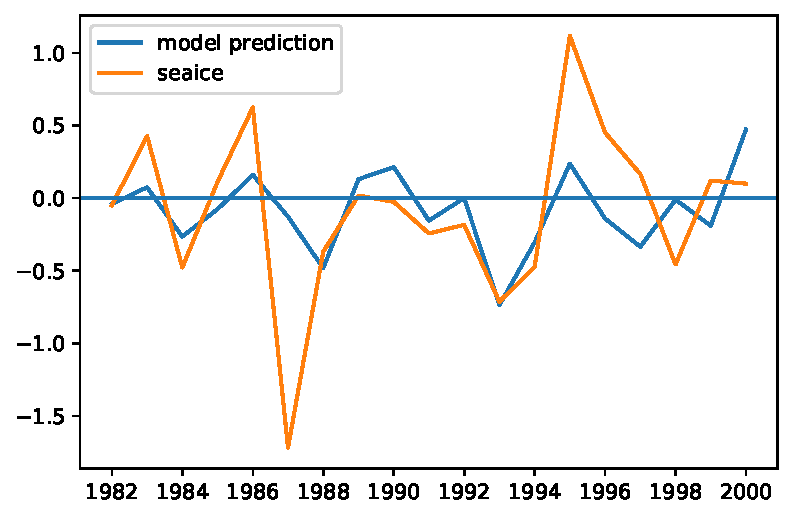
\includegraphics{Images_3.0/regressions/multivariate_model_anomalous_n1_annually_detrended_1979_2000.pdf}
    \caption{Fitted model for SIE detrended and averaged annually from 1979 to 2000.}
    \label{fig:multivariate_model_anomalous_n1_annually_detrended_1979_2000}
    \end{subfigure}
    
    \begin{subfigure}{\linewidth}
    \centering
    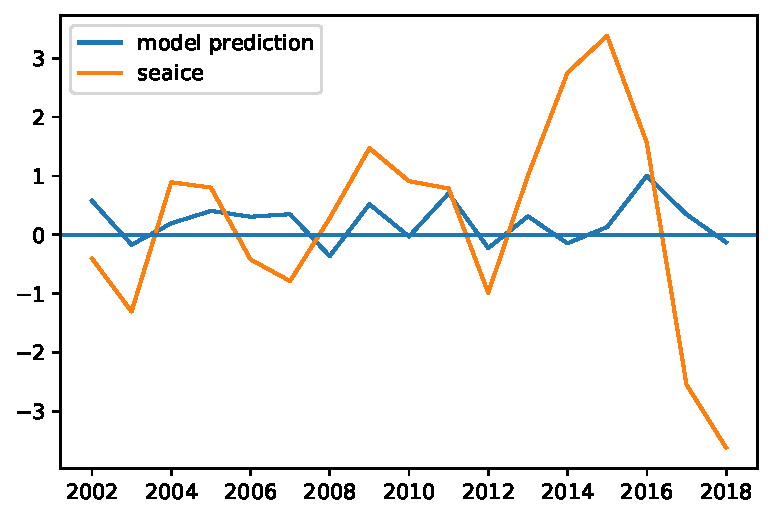
\includegraphics{Images_3.0/regressions/multivariate_model_anomalous_n1_annually_detrended_2001_2018.pdf}
    \caption{Fitted model for SIE detrended and averaged annually from 2001 to 2018.}
    \label{fig:multivariate_model_anomalous_n1_annually_detrended_2001_2018}
    \end{subfigure}
    \caption{Fitted model for SIE detrended and averaged annually. Before and after December 2000.}
\end{figure}

Likewise to looking at the entire time period, these plots are also demonstrating a bad fitting \textcolor{red}{put these in the same plot for easier comparison?}. For the same reasons as before this is unsurprising.

\newpage
\section{Spatial Regressions}
Looking at the regression analysis with the mean SIE we note that most of our fittings are not of great quality or statistically significant. We hope by introducing a spatial component to our analysis we can produce better quality results and begin to develop a more physical understanding of how these circulations impact the variability of sea ice in Antarctica.
Like before we start by doing individual regressions with each index we are interested in.
\begin{figure}[H]
    \centering
    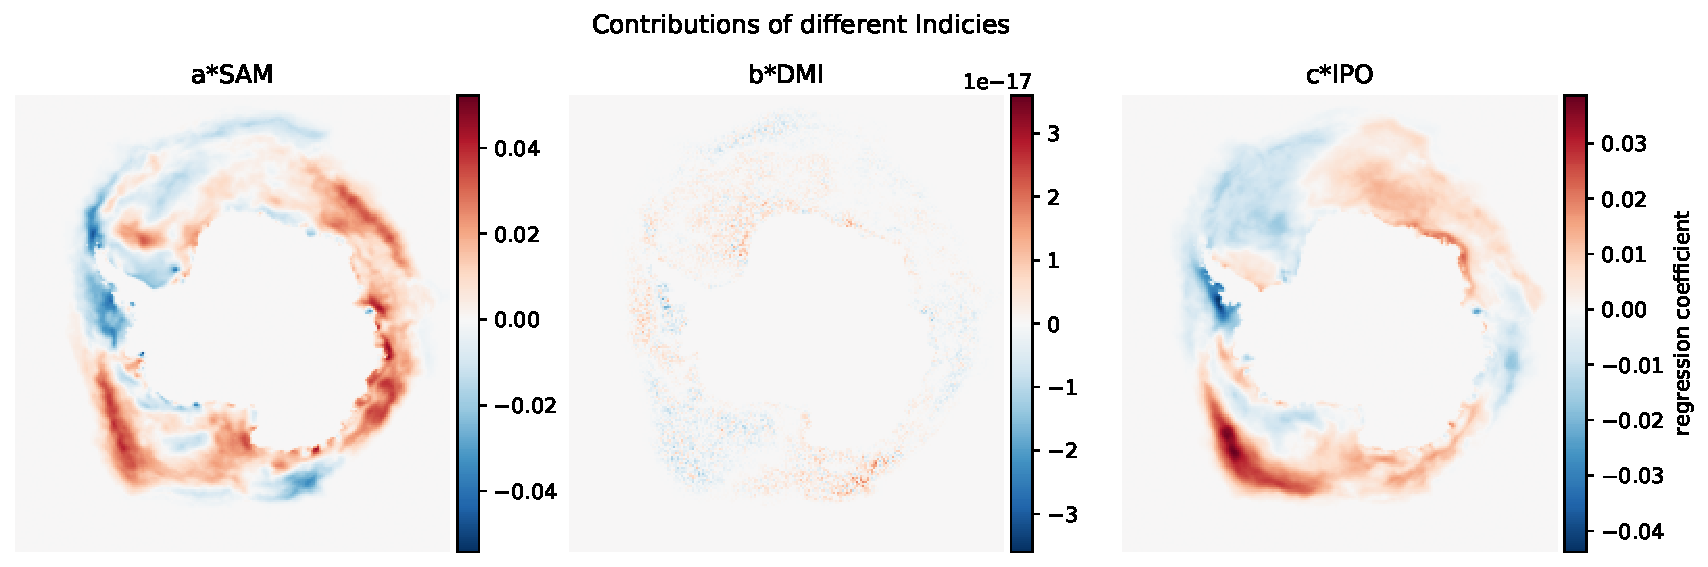
\includegraphics[width=\linewidth]{Images_3.0/regressions/index_contribution_anomalous_n1_annually_1979_2018.pdf}
    \caption[Spatial distribution of regression of SIC for each of the indices for 1979 to 2018]{Spatial distribution of regression of SIC for each of the indices for 1979 to 2018. Blue indicates a negative contribution and red indicates a positive contribution.}
    \label{fig:index_contribution_anomalous_n1_annually_1979_2018}
\end{figure}
Looking at these plots there are two main things which are notable. The first is that the expected contribution by DMI is much lower than the other two circulation patterns. For SAM this makes sense as it is localised around Antarctica. For IPO it also makes sense as the circulation is based over the Pacific \textcolor{red}{link this to the literature review.} The other thing to note is that the contribution of SAM and IPO are spatially very similar. This is interesting as we hypothesised that they impact the sea ice in Antarctica in different ways. It looking like SAM was more impactful for long term trends and IPO was more impactful for short term variability. This may or may not be the case. To understand this further we will need to look at the literature. As before this is done with a linear fitting, as such we don't expect the patterns here to indicate more that the base relationship that exists between these circulations and the behaviour of Sea ice in and around Antarctica. Likewise to before we will perform this same analysis, splitting the time series at the end of 2000, when IPO is noted to change it's overall phase. This can be seen below.

\begin{figure}[H]
    \begin{subfigure}{\linewidth}
    \centering
    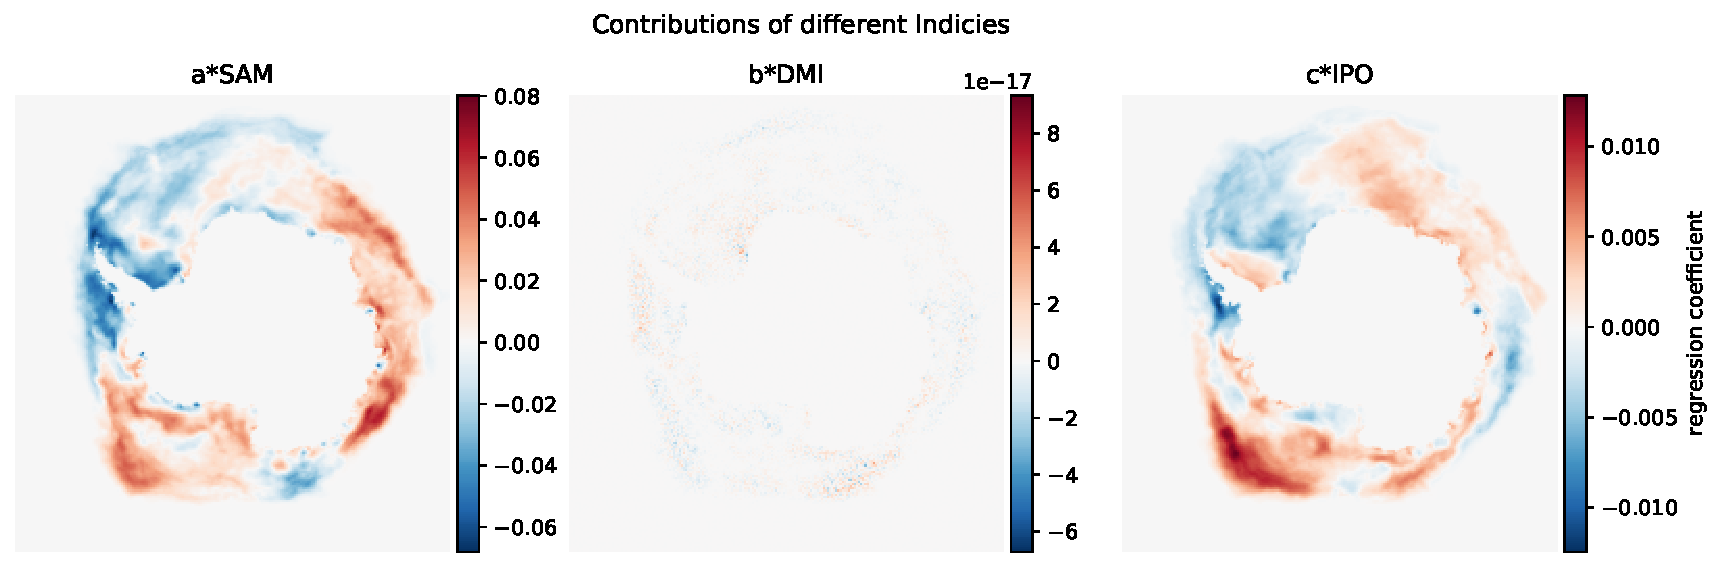
\includegraphics[width=\linewidth]{Images_3.0/regressions/index_contribution_anomalous_n1_annually_1979_2000.pdf}
    \caption{Spatial distribution of regression of SIC for each of the indices for 1979 to 2000.}
    \label{fig:index_contribution_anomalous_n1_annually_1979_2000}
    \end{subfigure}
    
    \begin{subfigure}{\linewidth}
    \centering
    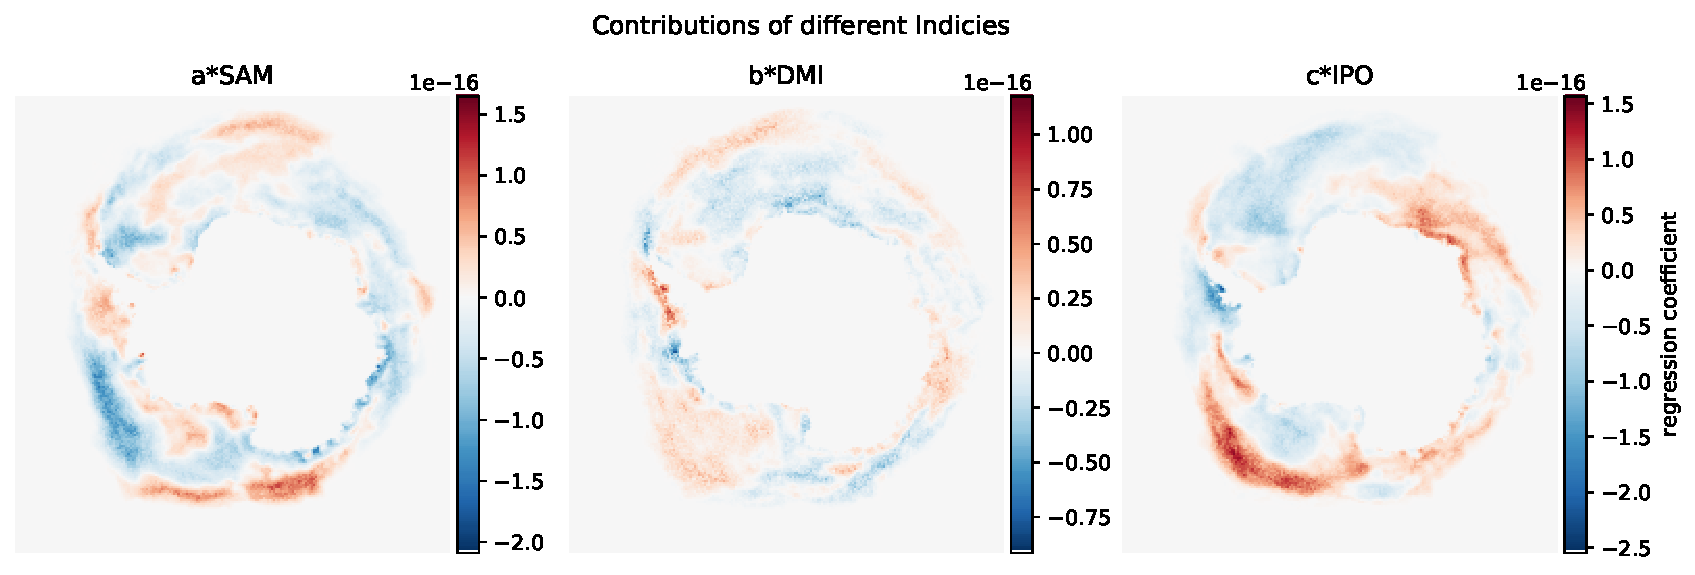
\includegraphics[width=\linewidth]{Images_3.0/regressions/index_contribution_anomalous_n1_annually_2001_2018.pdf}
    \caption{Spatial distribution of regression of SIC for each of the indices for 2001 to 2018.}
    \label{fig:index_contribution_anomalous_n1_annually_2001_2018}
    \end{subfigure}
    \caption{Spatial distribution of regressions for SIE for the different time periods in our dataset.}
\end{figure}
\newpage
\section{Variability of expected sea ice extent}
Considering the anomalous seasonal prediction, we can evaluate how good our model is with respect to the interannyal variability by plotting the expected sea ice extent against the true sea ice extent. In this case we ignore the time axis and plot the two ice extents together. We get the below plot.

Here wee can see that the model only accounts for about 5\% of the variability of sea ice extent in Antarctica with only a 0.22 pearson correlation coefficient between the two time series. This is unsurprising because the model is only fitting linearly and the system is much more complex and we expect non-linear relationships between global climate and the behaviour of sea ice in Antarctica. We do however find that the model fits the total sea ice extent with statistical significance, (a p-value of 0.01) Consequently we can see that while the model doesn't account for a large proportion of variability, the variability it expresses still contains useful information.

Considering the anomalous annual sea ice extent prediction, we notice that the gradient has increased to 5\% of variability being explained by our model. This also has a higher pearson correlation coefficient of 0.28, however the relationship isn't statistically significant with a p-value of 0.09. This will be due to the smaller number of data points. 

%%TC:ignore

%%%%%%% Bibliography %%%%%%%
\bibliographystyle{agsm}
\bibliography{references}

\part{Appendicies}
\appendix

\chapter{List of notation}
\begin{table}[H]
% \centering
\begin{tabular}{@{}r|l@{}}
\toprule
\textbf{Symbol} & \textbf{Meaning} \\ \midrule
    DJF & December, January, and February $\approx$ \textit{Summer}. \\
    MAM & March, April, and May $\approx$ \textit{Autumn}. \\
    JJA & June, July, and August $\approx$ \textit{Winter}. \\
    SON & September, October, and November $\approx$ \textit{Spring}. \\
    $r_{xy}$ & Pearson correlation coefficient. \\
    SIE & Sea Ice Extent. \\
    SIC & Sea Ice Concentration. \\
    ENSO & El Ni\~no Southern Oscillation. \\
    PDO & Pacific Decadal Oscillation. \\
    IPO & Interdecadal Pacific Oscillation. \\\bottomrule
\end{tabular}
\end{table}

% Don't count these!

\chapter{Word Counts}
\quickwordcount{main}
% \detailtexcount{main}

%%TC:endignore
\end{document} 